%%%%%%%%%%%%%%%%%%%%%% Props %%%%%%%%%%%%%%%%%%%%%%
\documentclass{article}

\usepackage[french]{babel}
\usepackage[utf8]{inputenc}
\usepackage[T1]{fontenc}
\usepackage{graphicx}
\usepackage{fancyhdr}
\usepackage{eurosym}
\usepackage{color}
\usepackage{soul}
\usepackage{listings}
\usepackage{enumitem}
\usepackage{enumerate}
\usepackage{float}

\pagestyle{fancy}
\lhead{Soutenance finale}
\chead{Deadly Science}
\rhead{Custos Carceris}

\definecolor{mygreen}{rgb}{0,0.6,0}
\definecolor{mygray}{rgb}{0.5,0.5,0.5}
\definecolor{mymauve}{rgb}{0.58,0,0.82}

\lstset{ 
  commentstyle=\color{mygreen},
  keywordstyle=\color{blue},       % keyword style
  numberstyle=\tiny\color{mygray}, % the style that is used for the line-numbers
  rulecolor=\color{black},         % if not set, the frame-color may be changed on line-breaks within not-black text (e.g. comments (green here))
  stringstyle=\color{mymauve},     % string literal style
  language=[Sharp]C,                 % the language of the code
  backgroundcolor=\color{white},   % choose the background color; you must add \usepackage{color} or \usepackage{xcolor}; should come as last argument
  basicstyle=\footnotesize,        % the size of the fonts that are used for the code
  breakatwhitespace=true,         % sets if automatic breaks should only happen at whitespace
  breaklines=true,
  extendedchars=true,              % lets you use non-ASCII characters; for 8-bits encodings only, does not work with UTF-8
  frame=single,	                   % adds a frame around the code
  tabsize=2,	                   % sets default tabsize to 2 spaces
  showstringspaces=false,
  numbers=left,
}

\begin{document}


%%%%%%%%%%%%%%%%%%%%%% Titre %%%%%%%%%%%%%%%%%%%%%%
\begin{titlepage}
	\centering
	{\scshape\LARGE Custos Carceris\par}
	\vspace{1cm}
	{\scshape\Large Rapport de projet\par}
	\vspace{1.5cm}
	{\huge\bfseries Deadly Science\par}
	\vspace{2cm}
	
\includegraphics[width=0.5\textwidth]{logo.png}\par\vspace{1cm}
	{\Large\itshape Léandre Perrot\par}
	{\Large\itshape Yann Boudry\par}
	{\Large\itshape Steve Suissa\par}
	{\Large\itshape Célian Raimbault\par}
	\vfill
	Un projet EPITA
	\vfill
	{\large \today\par}
\end{titlepage}



\newpage
\tableofcontents


%%%%%%%%%%%%%%%%%%%%% Intro %%%%%%%%%%%%%%%%%%%%%%

\newpage
\section{Introduction}
Depuis le début de l'année, notre groupe a travaillé sur ce projet, qui est aujourd'hui fini. De plus nous avons pu rajouter bien plus de choses que ce que le cahier des charges demandait, c'est-à-dire :

\begin{itemize}
\item Un autre mode de jeu que celui de base nommé le mode Nocturne, où toutes les lampes du laboratoire sont éteintes et où le joueur ne peut voir que grâce à sa lampe torche,
\item un système de paramètres de la partie permettant de choisir:
\begin{itemize}
\item la taille du labytinthe parmis plusieurs tailles prédifinies, où l'on peut choisir une taille personnallisée,
\item le nombre de joueurs dans la partie
\item le mode de jeu.
\end{itemize}
\item une cinématique dans le menu principal,
\item une refonte graphique totale des menus pour mieux coller à l'atmosphère du jeu et pour un meilleur rendu visuel, 
\item plus de 20 œufs de pâques cachés dans le jeu,
\item plus de 13 objets différents et bien plus!
\end{itemize}

Evidemment, tout cela sera expliqué par la suite. On notera que nous n'avons pas été en retard durant toute la durée du projet, car les seules tâches sur lesquelles on était légèrement en retard étaient largement comblé par le reste.

Nous sommes très fiers et confiants en notre projet. D'ailleurs nous allons le continuer pendant les vacances d'été tellement notre attachement sur le projet est grand. Ce fut un immense défi, que ce soit parce qu'il diffère largement d'un jeu de labyrinthe lambda, ou que ce soit pour la programmation car il nous a fallu comprendre et utiliser de nouveaux outils comme Unity ou Photon. Il a aussi fallu tout synchroniser en réseau, surtout que nous avons voulu faire un réseau plus large que nécessaire.

Le projet a été déjà grandement crée lors des deux premières soutenances, ces derniers mois n'ont servis qu'a peaufiné le tout, résoudre des bugs...

D'ailleurs pour réduire le plus de bugs, on a décidé de regrouper plus de 8 testeurs sur notre jeu en version alpha que l'on a réuni sur un salon dédié.

\newpage
\section{Reprise du cahier des charges}
\subsection{Eléments}
\paragraph{Caméra}
Chaque joueur doit avoir une caméra, elle doit représenter un angle de vue humain de 180 degrés. Elle doit donc prévenir et arrêter les mouvements de caméra impossible pour un humain comme par exemple pouvoir regarder derrière la tête.

\paragraph{Déplacements}
Chaque joueur doit pouvoir se déplacer dans toutes les directions. Il faut pouvoir facilement changer les vitesses, frictions en fonction de l'avancement du projet. Il peut aussi donner des coups de poing, qui baissent la barre d'endurance du joueur en face.

\paragraph{Endurance}
Les joueurs ont au dessus de leur tête leur pseudo, coloré en fonction de leur statut, et une barre d'endurance qui descend en fonction des dommages encaissés. Lorsque celle-ci est vide, le joueur avance plus lentement et la barre devient grise et se recharge progressivement. 

\paragraph{Statuts}
Lorsqu'un joueur est corrompu, il faut voir si un joueur guéri n'est pas trop près de lui, sinon lui aussi devient corrompu et doit aller contaminer les autres joueurs.

\paragraph{Phases}
Lorsque tous les joueurs sauf un ont ramassé les sérums, la deuxième phase du jeu doit commencer. Le dernier joueur doit devenir corrompu et il faut aussi s'assurer que tous les joueurs soient soit guéri, soit corrompu, soit invisible. La partie doit se terminer lorsque tous les joueurs sont infectés, et l'on doit afficher un écran de victoire si l'on gagne, et un écran de défaite si ça n'est pas le cas.

\paragraph{Sérums}
Les sérums peuvent être pris par les joueurs pour se guérir. Il faut faire attention à ce qu'un joueur corrompu ou guéri ne puisse pas prendre de sérum, et que les sérums sont bien détruits lorsqu'ils sont ramassés. Il faut aussi faire attention pour qu'il y ait exactement le bon nombre de sérums dans le labyrinthe, c'est-à-dire le nombre de joueurs moins 1.

\paragraph{Labyrinthe}
Le jeu doit contenir un labyrinthe assez grand pour pouvoir se perdre. Il faut aussi mettre plusieurs salles différentes pour un meilleur gameplay et pour mieux se perdre. Chaque salle doit avoir des meubles divers spécifiques, avec des modèles différents. Il doit être généré aléatoirement de manière à ce qu'on ait un labyrinthe différent quasiment à chaque fois que l'on crée une nouvelle partie. Il faut aussi faire attention à ce que les sérums se génèrent à l'intérieur du labyrinthe.

\paragraph{Modèles}
Chaque composants du labyrinthe doit avoir un modèle particulier, que ce soit les joueurs, les sérums, les meubles et différents objets des salles et tous les autres objets aussi.

\paragraph{Menus}
Il faut un menu principal, un menu pour créer la salle, la rejoindre, et la quitter. Le menu principal doit contenir un bouton pour commencer le jeu, et un bouton pour le quitter. Dans le second menu, il faut pouvoir accéder aux différents joueurs présents dans la salle puis pouvoir commencer la partie lorsque tous les joueurs sont prêts.

\paragraph{Réseau}
Le jeu doit être jouable en réseau, les effets des sérums doivent être synchronisés sur tous les joueurs, ainsi que la phase de la partie. Il faut aussi associer une caméra à chaque joueur, et faire attention qu'il y'en assez pour tout le monde, mais pas trop non plus! 

\paragraph{Site Web}
Il faut un site Web clair et net et esthétiquement plaisant à regarder. Il doit comporter les informations sur notre groupe, les liens pour télécharger les rapports de soutenance, de projet et le jeu. Il faut aussi qu'il contienne les règles et des images du jeu pour avoir une idée du jeu.

\paragraph{Effets}
Le jeu doit également être agréable à jouer, pour cela il est important d'ajouter plusieurs effets sonores et visuels tel que des musiques, bruitages, particules et plus...

\newpage
\subsection{Répartition des tâches}

\subsubsection{Célian}

Dans ce projet, je suis chargé principalement du gameplay du joueur ainsi que des effets visuels et sonores.

Avant d'entrer dans les détails des implémentations, voici la répartition des ajouts principaux que j'ai apportés au jeu :

\paragraph{Soutenance 1}

\subparagraph{Gameplay : joueur}

\begin{itemize}
    \item Physiques
    \item Mouvements du joueur
    \item Sérums
    \item Modules du joueur
\end{itemize}

\subparagraph{Gameplay : jeu}

\begin{itemize}
    \item Status
    \item Endurance et régénération
\end{itemize}

\subparagraph{Modèle et animations}

\begin{itemize}
    \item Modèle du joueur et animations (par des packages Unity)
    \item Animator et transitions
\end{itemize}

\paragraph{Soutenance 2}

\subparagraph{Phases et status}

\begin{itemize}
    \item Status local (les sérums affectent le joueur)
    \item Synchronisation du status à distance
    \item Evénements du joueur en réseau
\end{itemize}

\subparagraph{Endurance et coups}

\begin{itemize}
    \item Couches physiques (filtrage de collisions)
    \item Détection de collisions par rayon
\end{itemize}

\subparagraph{Gestion de l'audio}

\begin{itemize}
    \item Gestionnaire audio
    \item Effets sonores (implémentation et ajouts en partie des sons)
    \item Musiques et transitions (ajout de toutes les musiques)
\end{itemize}

\paragraph{Soutenance 3}

\subparagraph{Effets audio}

\begin{itemize}
    \item Ajouts d'effets sonores
    \item Sons en réseau
\end{itemize}

\subparagraph{Particules}

\begin{itemize}
    \item Gestionnaire de particules
    \item Particules de status
    \item Particules de coups
\end{itemize}

\subparagraph{Effets visuels}

\begin{itemize}
    \item Shaders sur la caméra
    \item Animation du shader
\end{itemize}

\subparagraph{Finalisation du jeu}

\begin{itemize}
    \item Désactivation des mouvements du joueur en pause
    \item Synchronisation du nom des joueurs (leur label)
    \item Status fantôme
    \item Changement de la taille des boîtes de collisions
    \item Désactivation des coups en assomé
\end{itemize}


\newpage
\subsubsection{Yann}

\paragraph{Soutenance 1}

\subparagraph{Menu principal}

\subparagraph{Paramètres}

\begin{itemize}
	\item Touches attribuables
	\item Sauvegarde
\end{itemize}

\subparagraph{"Pause"}

\begin{itemize}
	\item "Arrêt" de la partie (ne peut plus bouger)
	\item Touches attribuables
	\item Sauvegarde
	\item Effet immediat
\end{itemize}

\subparagraph{Début du site}

\paragraph{Soutenance 2}

\subparagraph{Modèles}

\begin{itemize}
	\item Croisement
	\item Impasse
	\item Intersection
\end{itemize}

\subparagraph{Ajout de paramètres}

\begin{itemize}
	\item Volume
	\item Effets sonores
	\item Sensibilité de la souris
\end{itemize}

\subparagraph{Rédaction du site}

\begin{itemize}
	\item Accueil
	\item Groupe
	\item Galerie
\end{itemize}

\paragraph{Soutenance 3}

\subparagraph{Video de fond sur le menu principal}

\subparagraph{Finalisation des paramètres}

\begin{itemize}
	\item Pseudo
	\item Langue
\end{itemize}

\subparagraph{Récapitulatif de la partie}

\subparagraph{Refonte des paramètres du labyrinthe}

Changement des boutons en commutateur pour surligner le paramètre actif

\subparagraph{Fin du site web}

\begin{itemize}
	\item Description des objets
	\item Évolution de jeu
	\item Image de fond
	\item Police
\end{itemize}


\newpage
\subsubsection{Steve}
\paragraph{Soutenance 1}
\begin{itemize}
    \item Caméra
    \item Système de génération des joueurs
    \item Menu de création de salle
    \item Menu de visualisation de la salle
    \item Synchronisation des postions des joueurs
\end{itemize}

\paragraph{Soutenance 2}
\begin{itemize}
    \item Optimisation des menus
    \item Système d'identification des joueus grâce aux RaiseEvents
    \item Identifications des joueurs locaux.
    \item Synchronisation des objets du labyrinthe en réseau
\end{itemize}

\paragraph{Soutenance 3}
\begin{itemize}
    \item Optimisation de la génération des joueurs
    \item Animation des joueurs en réseau
    \item Ajout des paramètres du labyrinthe
    \item Refonte graphique de tous les menus de connection.
    \item Ajout de précaution sur les menus et joueurs
    \item Carte en réseau
    \item Résolution de bugs
\end{itemize}

\newpage
\subsubsection{Léandre}
\paragraph{Soutenance 1}
\begin{itemize}
    \item Cénération du Labyrinthe
    \item Génération des Sérums
    \item Génération des emplacements des joueurs
    \item Construction du Labyrinthe en Blocs, et en Salles
\end{itemize}

\paragraph{Soutenance 2}
\begin{itemize}
    \item Composition de Thèmes Musicaux
    \item Construction des différents modèles 3D
    \item Debut de la mise en place des Plafonds
    \item Génération des Sérums en fonction des Joueurs
    \item Ajout de la possibilité de changer le nombre de joueurs, notamment pour jouer seul, avec le nombre de Sérums qui varie en conséquence
\end{itemize}

\paragraph{Soutenance 3}
\begin{itemize}
    \item Affichage des informations du joueur à l'écran
    \item Finitions des modèles 3D
    \item Instanciation des Lumières
    \item Ajout du Mode Nocturne
    \item Ajout de message d'erreur pour l'instanciation d'un labyrinthe aux dimensions personnalisées
    \item Génération de la Carte
    \item Génération des Objets
    \item Effets des différents Objets
\end{itemize}
\newpage
\section{Présentation du projet}
%%%%%%%%%%%%%%%%%%%%%% Yann %%%%%%%%%%%%%%%%%%%%%%%%%%%%%%%%%%%%%%%%%%%%%%%%%%%%%%%%%%%%%%%%%%%%%%%%%%%%%%%%%%
\subsection{Yann}
\subsubsection{Menu principal}

Le menu est la première image qu'aperçoit le joueur du jeu. Il est important d'avoir un menu bien réalisé et qui donne envie de jouer à l'utilisateur. Chose promise, chose due, la couleur de fond a été remplacée par une video de présentation du jeu, et le nom du jeu est présent aussi, c'est tout de même mieux avec.

\begin{figure}[!h]
	\centering
	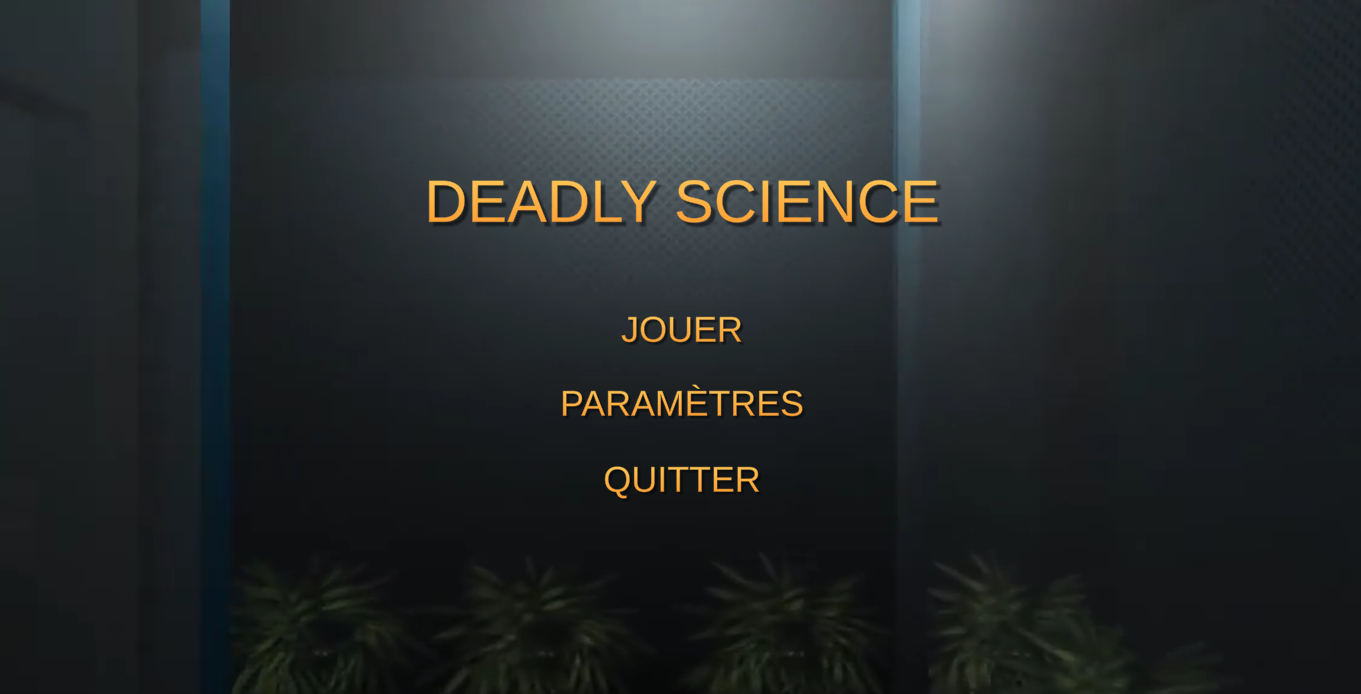
\includegraphics[width=0.8\textwidth]{MainMenu.png}
	\caption{Menu principal}
	\label{Menu principal}
\end{figure}

\paragraph{Accueil}
J'ai créé la vidéo avec l'asset d'animation d'Unity. Le défi a été d'enregistrer cette video puisque les animations faites de cette manière requièrent l'environnement sur la scène. En effet la caméra bouge ainsi d'elle même selon l'enregistrement effectué et l'utilisateur n'a aucun contrôle dessus. Cependant dans notre jeu le labyrinthe est généré sur une autre scène que le menu et seulement lorsqu'une partie est commencée. Or il est impossible de sauvegarder une animation en mode jeu dans Unity. Il a donc fallu créer toute l'animation en une seule fois et j'ai enregistré l'écran en la jouant. Après un léger recadrage, c'est un composant de lecture video qui affiche l'enregistrement en boucle dès le lancement du jeu.
\newline
Le menu permet donc de commencer une partie, d'acccéder aux paramètres ou de quitter le jeu. Il serait triste de quitter maintenant alors qu'il vient d'être lancé, alors continuons.

\paragraph{}
Vous pouvez dès à présent commencer une partie dans l'univers de Deadly Science, avec vos amis, ou en joignant une salle créée par quelqu'un d'autre. Mais si les paramètres vous intriguent, allez donc y jeter un oeil.

\paragraph{Paramètres}
(Menu principal)

\begin{figure}[H]
	\centering
	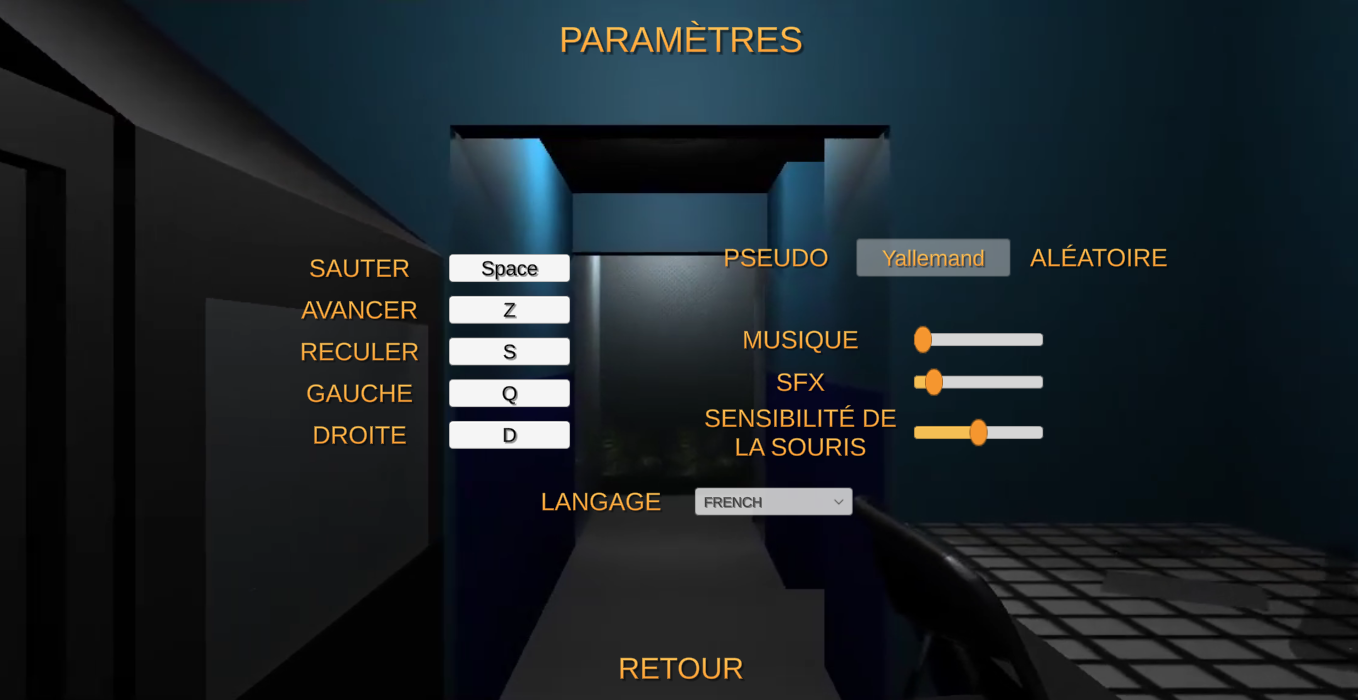
\includegraphics[width=0.8\textwidth]{Parametres.png}
	\caption{Paramètres}
	\label{Paramètres}
\end{figure}

Seul le canvas change pour accéder aux pramètres, ce qui permet de garder la video en fond sans interruption.
Vous trouverez centré en bas de paramètres, le langage du jeu, qui permet de choisir entre Français ou Anglais. Le changement est effectif immédiatement et sauvegardé pour les prochaines scènes et arties. Ce paramètre a été réalisé à l'aide d'un asset de l'asset store de Unity nommé Language Localization. Après quelques modifiacations permettant de l'apliquer aux zones de texte Text Mesh Pro, il fontionne parfaitement bien. Il permet de créer des dictionnaires
\subparagraph{}
Sur la gauche de ce menu se trouve le gestionnaire de touche du jeu. A côté de chaque action se trouve un bouton contenant la touche associée à cette action. Pour la changer, il suffit de cliquer sur le bouton et la première touche enfoncée sur le clavier est donc attribuée à cette action. Cela se fait simplement en analysant chaque touche du clavier une par une et en trouvant celle qui est enfoncée. Un script permettait auparavant d'instancier chaque action et son bouton associé mais cette utilisation aurai rendu compliqué le changement de langue au chargement du jeu. En effet les touches sont stockées à l'aide d'un dictionnaire, changer les noms des entrées réinitialiserai le dictionnaire, or le joueur n'a pas envie de refaire tous ses paramètres à cause d'un changement de langue.

\subparagraph{}
A droite, vous pouvez trouver une zone de texte qui correspond à votre pseudo en jeu, transmis aux autre joueurs de la partie. Il est également possible de prende un pseudo aléatoire qui est constitué du mot "sujet" et d'un nombre entre 1000 et 9999. Nous avons opté pour cela car rappelons-le nous sommes dans un laboratoire expérimental. De plus le pseudo aléatoire est adapté au langage puisque "sujet" est remplacé par "subject" en Anglais.

\subparagraph{}
Finalement dans la partie en bas à droite de trouvent trois slider permettant de régler respectivement le volume de la musique, des effets sonores et la sensibilité de la souris.

\begin{itemize}
	\item{Le volume de la musique} correspond bien entendu à la musique du jeu qui permet d'approfondir l'expérience du joueur et contribue à l'ambiance lugubre du jeu. Il prend une valeur entre 0 et 1, ce qui correspond donc à couper totalement la musique ou mettre le volume au maximum.
	\item{Le volume des effets sonores} correspond à tous les autre sons du jeu, instantanés et courts, tels que les bouton ou les coups porté entre les joueurs. Il est également compris entre 0 et 1, correspondant à la même interprétation: aucun son, ou le maximum.
	\item{La sensibilité de la souris} permet, sans grosse surprise de régler la vitesse de la souris dans le jeu, qui est associé à la rotation du personnage. Elle a une plage de valeur plus petite, entre 0.1 et 0.7. Le minimum est à 0.1 car je ne voulais pas que les joueurs puissent empêcher la rotation du personnage et de la caméra, et le maximum est à 0.7 car au delà, le jeu devenait injouable car la caméra était incontrolable. Le joueur rentrait alors dans tout les murs et ne pouvait qu'à peine changer de salles.
\end{itemize}

\subsubsection{Ecran de "pause"}
Un écran de "pause" (c'est un jeu multijoueurs, il n'y a pas vraiment de pause) s'ouvre lorsque le joueur appuie sur la touche "echap". La souris apparait alors et il devient impossible de se déplacer.

\begin{figure}[H]
	\centering
	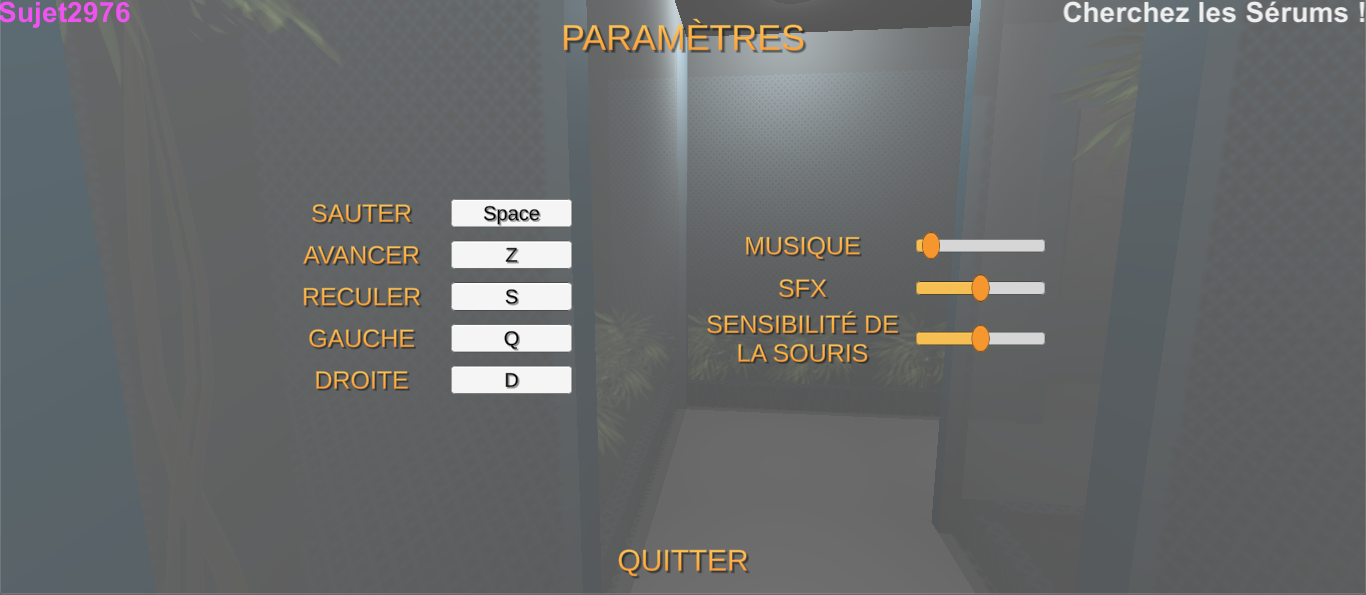
\includegraphics[width=0.8\textwidth]{Pause.png}
	\caption{L'écran de "pause"}
	\label{L'écran de "pause"}
\end{figure}


On y retrouve certains paramètres: les touches pour jouer, le volume de la musique, des effets sonores et la sensibilité de la souris. pour des raisons évidentes d'identification, il est impossible de changer son pseudo en cours de partie. De même, la langue du jeu est seulement modifiable sur le menu principal. Pour quitter la fenêtre, il suffit de réappuyer sur la touche "echap", la souris disparait et le joueur peut de nouveau contrôler son avatar.

\subsubsection{Écran de fin}
\paragraph{Deux possibilités:}
Soit le joueur est le premier condamné et à réussi à infecter tous les autres, ou le joueur à réussi à survivre toute les durée de la partie, il gagne et est notifié par un magnifique "Victoire" vert. Soit il était soigné mais a été réinfecté et meurt donc dans l'indifférence la plus totale du joueur qui s'empresse de relancer une autre partie. Il est alors notifié d'un "Défaite" rouge. Dans les deux cas il est impossible de se déplacer lorsque la partie est terminée. A cela s'ajoute un récapitulatif de la partie au centre de l'écran. Il y est inscrit chaque évênement auquel le joueur à fait face, le soin, la contamination, les différents objets rammassés. A chaque évênement, une nouvelle zone de texte est créée et se rajoute à la liste.

\begin{figure}[H]
	\centering
	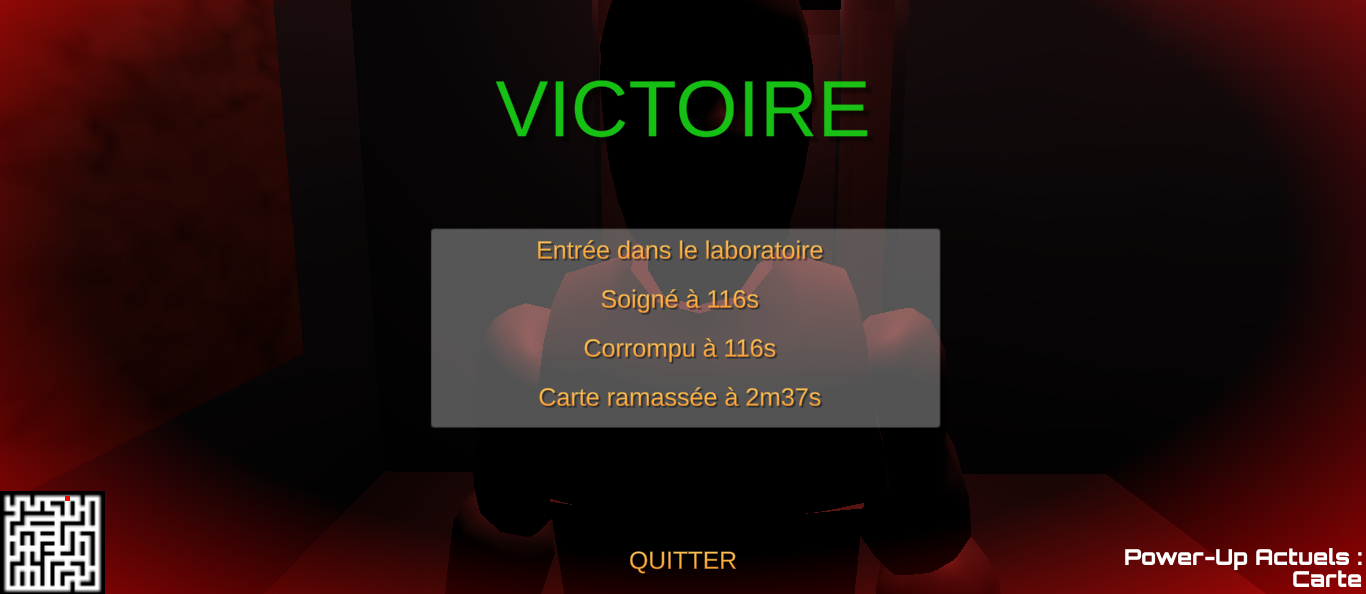
\includegraphics[width=0.49\textwidth]{Victoire.png}
	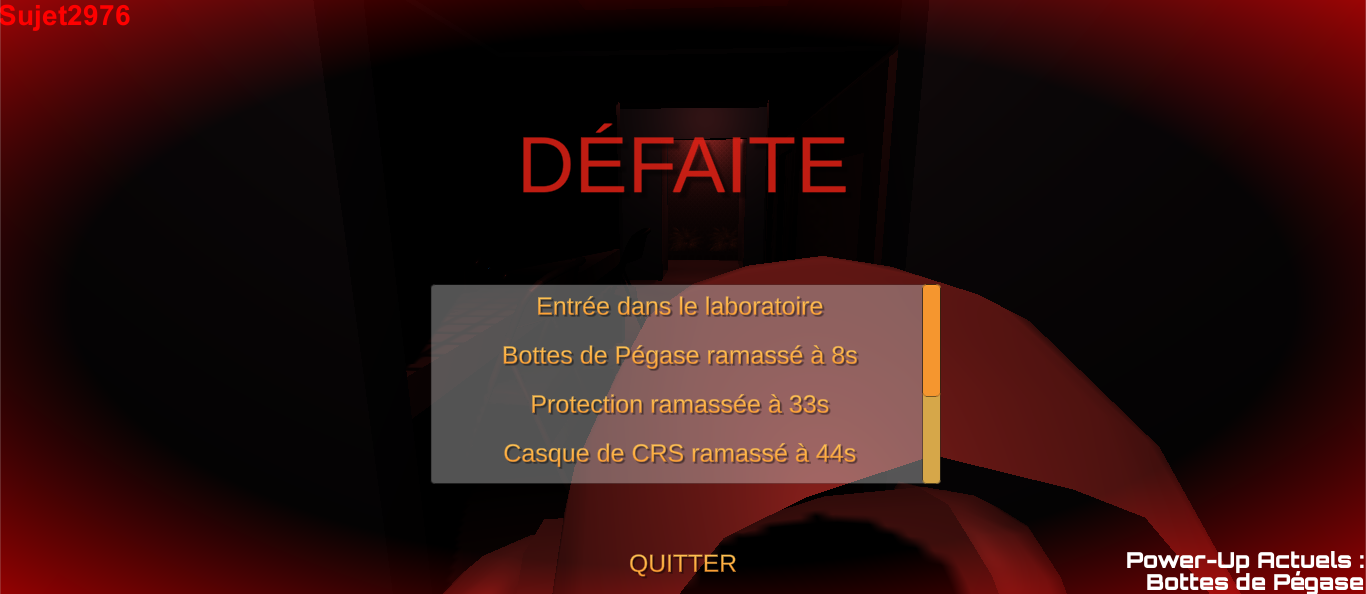
\includegraphics[width=0.49\textwidth]{Defaite.png}
	\caption{Écrans de fin}
	\label{Écrans de fin}
\end{figure}

\subsubsection{Site Web}
Le site web se présente en 5 pages différentes:
\begin{itemize}
	\item{} L'accueil ( ou projet) qui présente le jeu.
	\item{} Le groupe qui constitue la présentation de chacun
	\item{} La galerie, collection de photos du jeu
	\item{} Le codex, qui rasssemble les objets du jeu
	\item{} La page de téléchargement
\end{itemize}
L'image de fond est identique sur toute les pages et montre une salle du labyrinthe.

\paragraph{L'accueil}présente Deadly Science, son origine et le déroulement d'une partie. Ce premier paragraphe est suivi de l'évolution du jeu entre les soutenances depuis la naissance du projet à cette dernière présentation.

\paragraph{Le groupe}présente chaque membre du groupe, accompagné de sa magnifique poto du CRI en médaillon.

\paragraph{La galerie}regroupe des photos de chaque salle utilisées dans le labyrinthe et développés par Léandre et moi. Vous trouverez en dessous des photos finales celles des anciennes versions du jeu.

\paragraph{Le codex}présente les objets de Deadly Science connus du public en trois catégories: ceux qui vous aident dans votre mission, ceux qui vous ralentisent dans votre mission et ceux qui... On ne sait pas trop à quoi ils servent en fait. Il seront plus amplement expliqués par la suite (ou vous pouvez allez voir le site).

\paragraph{L'onglet de téléchargement}permet en accord avec toutes les probabilités, de télécharger le jeu, ainsi que les différents documents (cahier des charges et rapports) réalisé pendant la durée du projet.


\subsection{Steve}
\newpage
%%%%%%%%%%%%%%%%%%%%%% Steve%%%%%%%%%%%%%%%%%%%%%%%%%%%%%%
Pour se connecter il y'a trois menus, le menu pour créer la partie, le menu pour changer les paramètres de la partie, et enfin le menu on peut voir les joueurs connectés et commencer la partie. Chacun des 3 menus ont subi une refonte graphique pour correspondre à l'ambiance du jeu et avoir un aspect visuel plus plaisant.

\subsubsection{Menu pour créer la partie}

Voici à quoi ce menu ressemble : 

\begin{figure}[!ht]
    \centering
    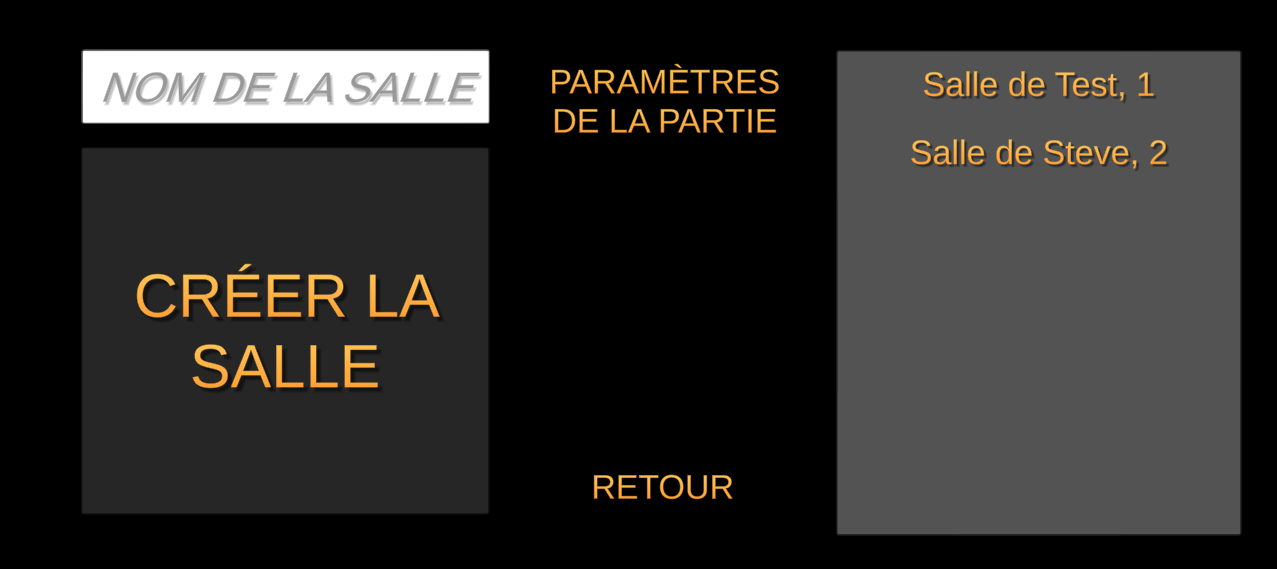
\includegraphics[width=0.8\textwidth]{Menu1.png}
    \caption{Menu pour créer la salle}
    \label{Menu pour créer la salle}
\end{figure}

Il est composé de deux parties. Celle de gauche on peut écrire dans la barre blanche le nom de la salle que l'on veut créer et un bouton "Créer la salle" qui comme son nom l'indique permet de créer la salle et d'entrer dans un autre menu que l'on verra par la suite. La partie droite liste chacune des salles avec leur noms et le nombre de joueurs déjà présents dans la salle. Elle est sur un tableau défilant ce qui permet d'avoir autant de parties que l'on souhaite. Cela permet de savoir si par exemple on va attendre plus ou moins longtemps avant le début de la partie. Pour rejoindre la salle que l'on souhaite, c'est simple, il suffit de cliquer dessus et cela nous fait rentrer dans la dite salle. A noter que si la salle est remplie à son maximum, elle ne sera pas montrée comme visible, vu qu'on ne peut pas la rejoindre. En ce qui concerne les deux boutons du milieu, le bouton "Retour" nous fait retourner à l'écran principal et le deuxième bouton nous transporte dans le menu des paramètres du labyrinthe que l'on va maintenant regarder.

\subsubsection{Menu pour les paramètres de la partie}

Ce menu ne sert que pour l'hôte de la partie, les autres joueurs n'ont pas besoin d'interagir avec celui-ci. Dans ce menu on peut changer de mode de jeu entre Classique et Nocturne (ces modes de jeu seront expliqués par la suite). On peut aussi changer le nombre de joueurs de la partie. Enfin on peut choisir la taille du labyrinthe parmis plusieurs dimensions prédéfinies ou bien choisir une taille personnalisée (par exemple un labyrinthe rectangulaire) en l'écrivant sur la barre blanche et confirmer. Pour sélectionner l'option que l'on souhaite, il suffit encore tout simplement de cliquer dessus. Par exemple sur la Figure 2, on peut voir que le mode de jeu choisi est Classique, que la salle peut contenir quatre joueurs et que la taille du labyrinthe est de dix en largeur et 10 en longueur. Lorsque l'on a choisi ses paramètres, il suffit d'appuyer sur le bouton "Retour" qui nous envoie sur le menu précédant et on peut créer la partie avec les paramètres enregistrés. On peut souligner que les modes de jeu et les tailles du labyrinthe sont sur des tableaux défilants, ce qui permet premièrement l'ajout de nouveaux modes ou de nouvelles tailles facile, mais aussi que l'on peut en ajouter autant qu'on veut, il suffit juste d'utiliser la molette de la sourie pour accéder aux options tout en bas.



\begin{figure}[!ht]
    \centering
    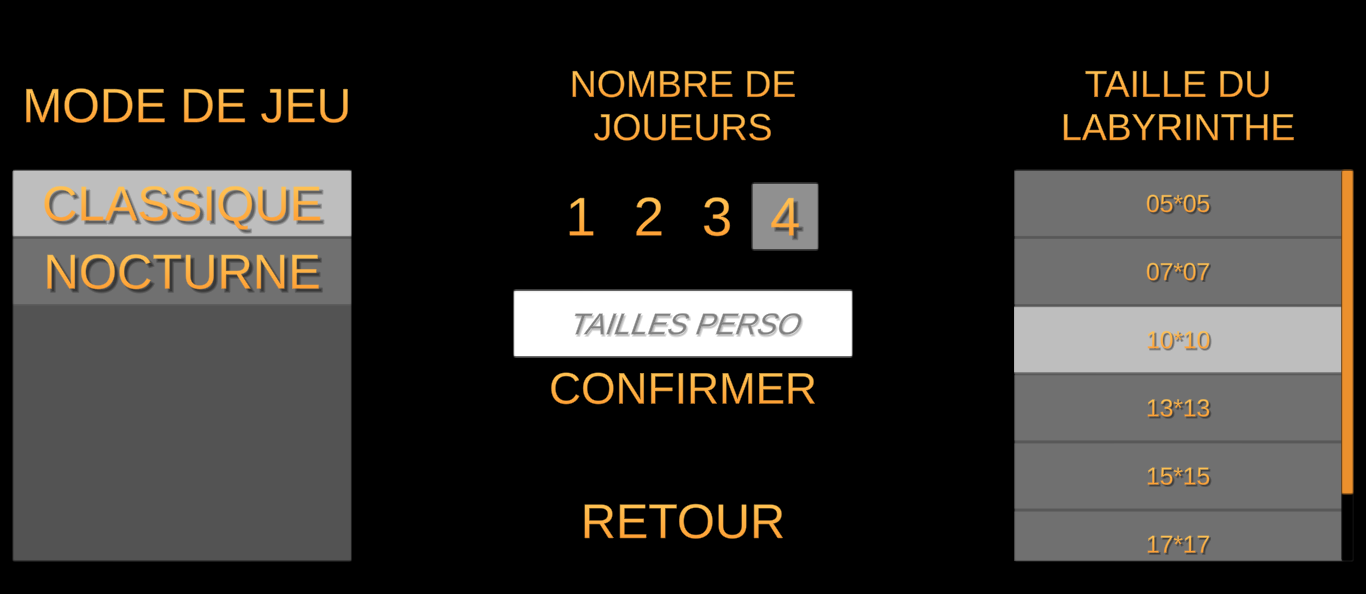
\includegraphics[width=0.8\textwidth]{Menu2.png}
    \caption{Menu pour les paramètres de la partie}
    \label{Menu pour les paramètres de la partie}
\end{figure}


\subsubsection{Menu pour commencer la partie}

Ce menu a la particuliarité d'être différend en fonction de notre rôle dans la partie. Si on est l'hôte de la salle, alors le bouton en bas à gauche est "Commencer" permettant de débuter la partie, et sinon il est nommé "Prêt" qui permet de savoir si chacun des joueurs est prêt à commencer la partie comme montré sur les Figures 3 et 4. D'ailleurs à droite, on peut voir la liste des joueurs avec leur pseudonyme et leur rôle. A nôter que l'actualisation des statuts des joueurs est quasiment instantané et que le bouton "Prêt" change si on est prêt ou pas. Si on ne l'est pas il sera renommé "Non Prêt". L'hôte ne peut commencer la partie que si chacun des joueurs, et chacun des joueurs entre dans la salle avec un statut "Non Prêt". Dès que le nombre de joueurs attendus correspond au nombre de joueurs dans la salle et que tous les joueurs sont prêts, l'hôte peut débuter la partie. Lorsque la partie commence, la salle n'est plus accésible ni visible. En dehors de ça, peu importe notre rôle, on peut décider à tout moment de quitter la salle en appuyant sur le bouton éponyme. Si l'on est hôte, tous les joueurs de la salle sont transportés dans le menu pour créer la salle. De plus, des protections ont été mises de manière à ce que même si, par exemple, l'hôte viendrait à cliquer sur le bouton "	Commencer" alors que tous les joueurs ne sont pas prêts, la partie ne débutera pas.

\newpage
\begin{figure}[!ht]
    \centering
    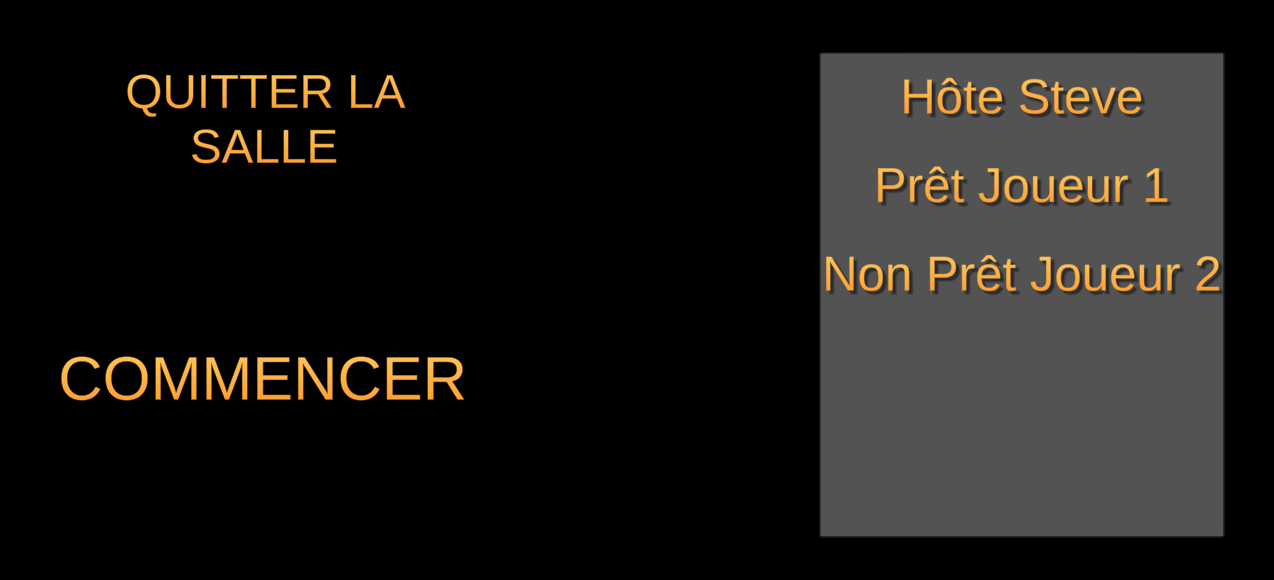
\includegraphics[width=0.8\textwidth]{Menu31.png}
    \caption{Menu lorsqu'on est hôte}
    \label{Menu lorsqu'on est hôte}
\end{figure}



\begin{figure}[!ht]
    \centering
    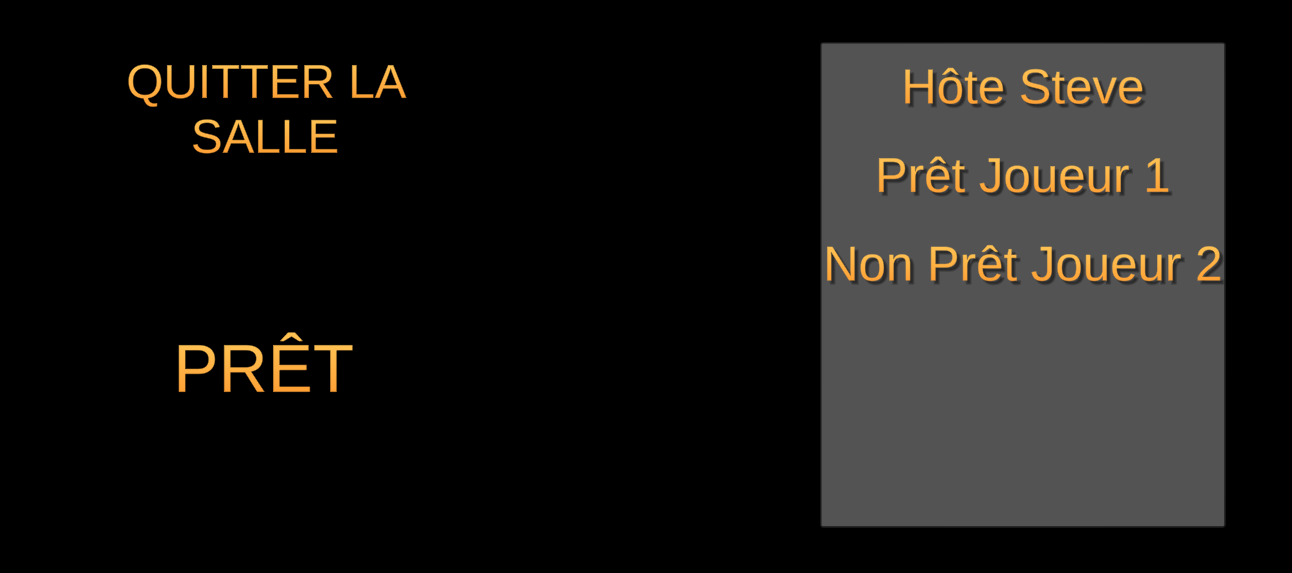
\includegraphics[width=0.8\textwidth]{Menu32.png}
    \caption{Menu lorsqu'on n'est pas hôte}
    \label{Menu lorsqu'on n'est pas hôte}
\end{figure}

\subsubsection{Réseau}
En dehors des menus et d'être chef de projet, j'ai été en charge de la gestion du réseau. Cela passe par la génération des joueurs, la synchronisation des objets 
etc... Il est dur de visualiser ou de comprendre les effets du réseau mais je vais faire de mon mieux pour le faire.

\paragraph{Génération des joueurs}

L'une des plus grandes difficultés du projet et c'est sans doute ce qui nous a pris le plus de temps. Le pire, c'est qu'au premier abord on pourrait croire que ça 
serait quelque chose de simple, il suffirait de mettre un identifiant à chacun des joueurs et en fonction de l'identifiant de l'instancier à la position que l'on 
souhaite. Malheuresement ce ne fut pas assez simple.

On a pensé premièrement à utiliser la variable LocalPlayer de Photon avec le dictionnaire des Players. Cela n'a 
pas fonctionné car tout les joueurs avaient les mêmes propriétés, c'est-à-dire mêmes pseudos, mêmes identifiants etc... On a cru pendant longtemps que c'était le 
LocalPlayer le problème mais avec nombreux tests, on sait rendu compte que c'était le dictionnaire qui ne marchait pas.

Après on a pensé à utiliser les RaiseEvents, mais c'était inutile pour ce que l'on cherchait à faire. On a après pensé à utilisé les PhotonViews mais le problème c'est 
que cela permettait de déterminer si on était le joueur mais pas par rapport aux autres. Or on cherchait un moyen de le distinguer des autres joueurs.

On a pensé à utilisé l'hôte de la salle (que l'on appelle aussi le MasterClient) comme base pour envoyer les messages de tous les joueurs, mais ce fut beaucoup très complexe et non 
performant. A la fin, on a utilisé les PhotonViews, les LocalPlayers et les RPCFonctions pour envoyer les messages en réseau. Cette méthode fut optimisée et parfaite 
pour ce que l'on cherchait.

\paragraph{Propritétés des joueurs}
La génération des joueurs ne concerne que la première partie du réseau, elle ne se lance qu'au début de la partie. Il reste ensuite à synchroniser les mouvements, 
rotations, animations des joueurs. Pour cela j'ai du utiliser les Photon Transform et Animator Views. Ce fut plus compliqué que attendu, vu que le joueur est consistué 
de plusieurs parties et il fallait que toutes soient synchronisé pour tout le monde. 

De plus, il fallait aussi cacher les animations au joueur qui les faisait car 
sinon les animations rencontrer la caméra ce qui n'était pas du tout le résultat souhaiter. Heuresement, avec beaucoup de recherche et de travail, tout est maintenant 
synchronisé au dixième de seconde, permettant des actions rapides pour dynamiser le jeu.

Sans vouloir rentrer dans les aspects techniques du code, ce fut l'essentiel de mon acitivité en dehors des menus. En dehors de ça, j'ai du me charger de synchroniser tout les travaux de tous mes collègues comme le labyrinthe par exemple, car sinon les joueurs ne sont pas dans le même labyrinthe. 


%%%%%%%%%%%%%%%%%%%%%% Celian %%%%%%%%%%%%%%%%%%%%%%%%%%%%%%%%%%%%%%%%%%%%%%%%%%%%%%%%%%%%%%%%%%%%%%%%%%%%%%%%%%
\subsection{Célian}



\newpage
\paragraph{Principe du jeu}


Notre jeu possède deux phases.
Premièrement, les joueurs sont des personnes ayant été infectées par une maladie. Ils doivent alors récupérer les échantillons de sérum ayant été dissimulés dans les souterrains du laboratoire qui étudie la maladie. Il n'y a malheureusement pas assez de sérums, une personne restera infectée. Pour éviter de le rester, vous devez chercher le plus vite possible un sérum dans le dédale.
Quand tous les sérums ont été consommés, une nouvelle phase commence. Il ne reste alors plus qu'une chance au condamné de gagner : en infectant les joueurs guéris. Les joueurs ayant pris des sérums doivent alors courir ou se cacher pour éviter de se faire attraper, au bout de quelques minutes, c'est la victoire des joueurs guéris - mais seulement s'il en reste - sinon seul le joueur qui n'a pas été guéri gagne.


%%% TODO : Parler gen labyrinthe


\subsubsection{Gameplay}


Une fois que vous êtes dans le labyrinthe,
Pour contrôler le joueur, il suffit d'appuyer sur les touches que vous avez enregistrées (ou WASD par défaut) pour les mouvements horizontaux ou sur espace pour sauter, concernant la caméra, la souris est utilisée. Nous pouvons également attaquer d'autres joueurs en appuyant sur le bouton gauche de la souris et en ayant un joueur devant nous.


%%% TODO : vvv Reformuler / Déplacer ?


Chaque joueur possède son nom au-dessus de sa tête, il sert d'une part à connaître quel joueur nous avons en face de nous, mais aussi sert à indiquer le statut du joueur par sa couleur qui est la même que celle de son statut.
Pour connaître son propre statut, nous pouvons regarder en haut à gauche de l'écran, notre nom est affiché avec la même couleur que celle de notre statut.


\subsubsection{Endurance}


Pour que le jeu soit plus intéressant, j'ai pensé à intégrer une jauge d'endurance.


L'endurance est semblable à une barre de vie dans la plupart des jeux, contrairement à une barre de vie, une fois vide, elle ne tue pas le joueur, mais le rend faible. Ainsi, le joueur se déplace très lentement (10\% de sa vitesse normale) et ne peut plus sauter. Il ne peut pas non plus attaquer ni reprendre de coup pour éviter qu'un joueur le bloque.


Cette jauge se remplit petit à petit et une fois le joueur assommé, il doit attendre que cette barre d'endurance se remplisse totalement avant de retrouver ses habilités.


\begin{figure}[H]
\centering
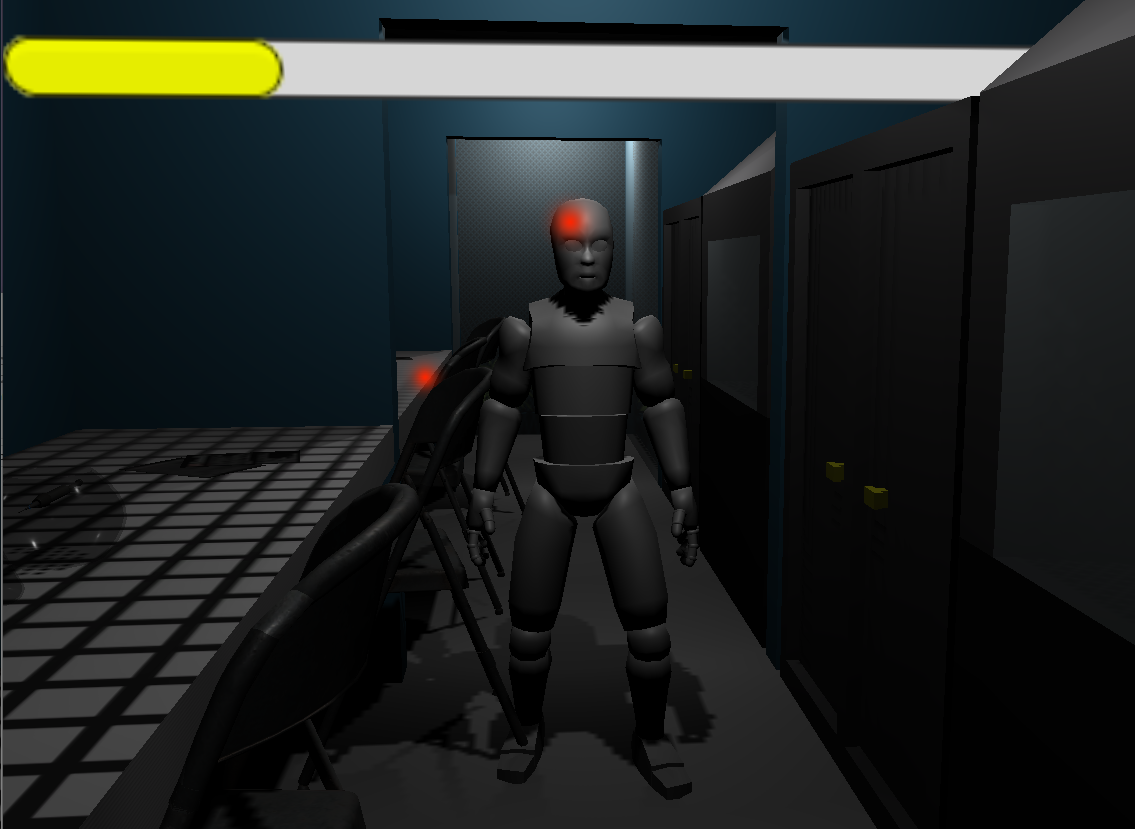
\includegraphics[width=0.8\textwidth]{cc/stamina.png}
\caption{Un joueur ayant pris des coups}
\label{cc_a}
\end{figure}


À présent, parlons de comment un joueur peut assommer un autre joueur, c'est très simple, à la manière d'un jeu de tir à la première personne, un joueur doit viser une cible puis cliquer avec sa souris. Bien sûr, il y a une portée maximale, car le joueur ne tire pas vraiment, c'est juste un coup. De plus, en seconde phase, si un joueur de statut condamné donne un coup à un autre joueur de statut guéri, celui-ci prend le statut condamné. Cette façon permet aux joueurs de plus facilement interagir entre eux.


Pour qu'un joueur puisse savoir si un autre joueur est assommé, une barre d'endurance est présente sur la tête de chaque joueur, elle devient grise une fois que le joueur est sonné.


\begin{figure}[H]
\centering
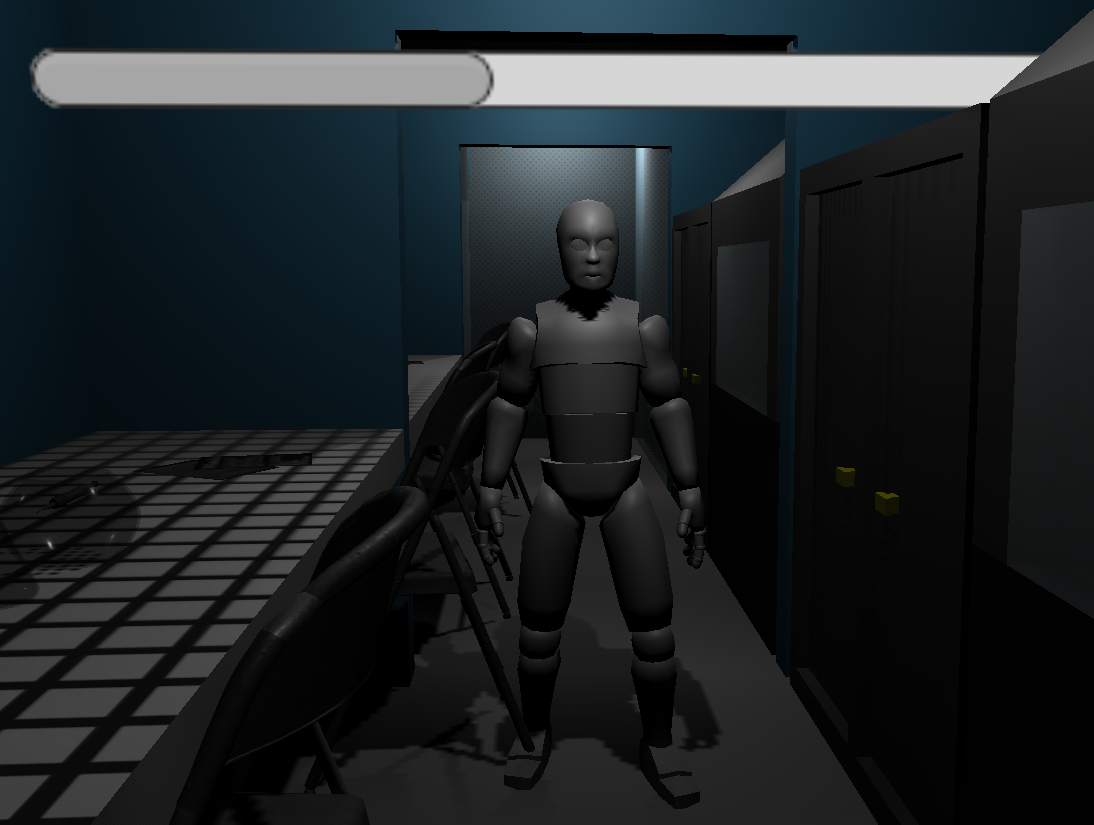
\includegraphics[width=0.8\textwidth]{cc/stamina_stunned.png}
\caption{Un joueur sonné}
\label{cc_b}
\end{figure}


\subsubsection{Effets audio}


Deadly Science dispose de divers effets audio pour renforcer l'ambiance du jeu.
Il y a des musiques lors du menu ou du jeu ainsi que des effets sonores joués lors d'une action faite par l'utilisateur. 
De plus, les musiques s'enchaînent avec des transitions et les effets sonores peuvent être joués en réseau.


\paragraph{Effets visuels}


En plus d'effets audio, Deadly Science possède des effets visuels supplémentaires, ils accompagnent les actions des joueurs au cours du jeu.


\paragraph{Particules}


Les particules sont présentes sous plusieurs formes.
Par exemple, lors d'un changement de statut, nous pouvons voir qu'un nuage de particules de la couleur du statut jaillit. Il possède plusieurs points colorés, certains ont aussi des traînées de la même couleur.
Elles sont également présentes lors d'un coup donné à un autre joueur.


\begin{figure}[H]
\centering
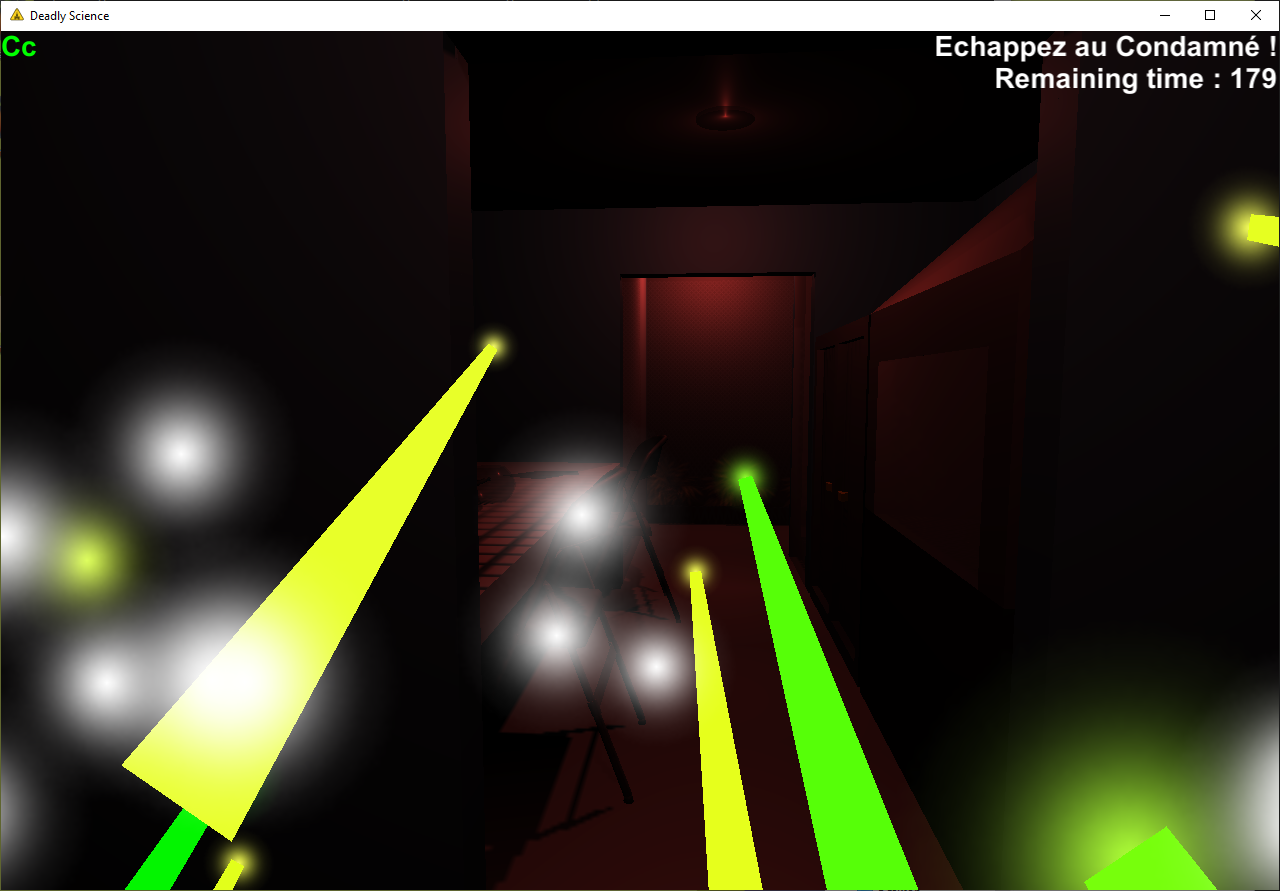
\includegraphics[width=0.8\textwidth]{cc/particles_example.png}
\caption{Des particules lors d'une prise de sérum}
\label{cc_c}
\end{figure}


\paragraph{Post-traitement}


Le joueur condamné en seconde phase a une lourde responsabilité, c'est pour cela qu'un effet de vignettage rouge fait apparition à l'écran.
Cet effet oppressant est animé à la façon d'un battement de coeur et dure jusqu'à la fin de la partie.


\begin{figure}[H]
\centering
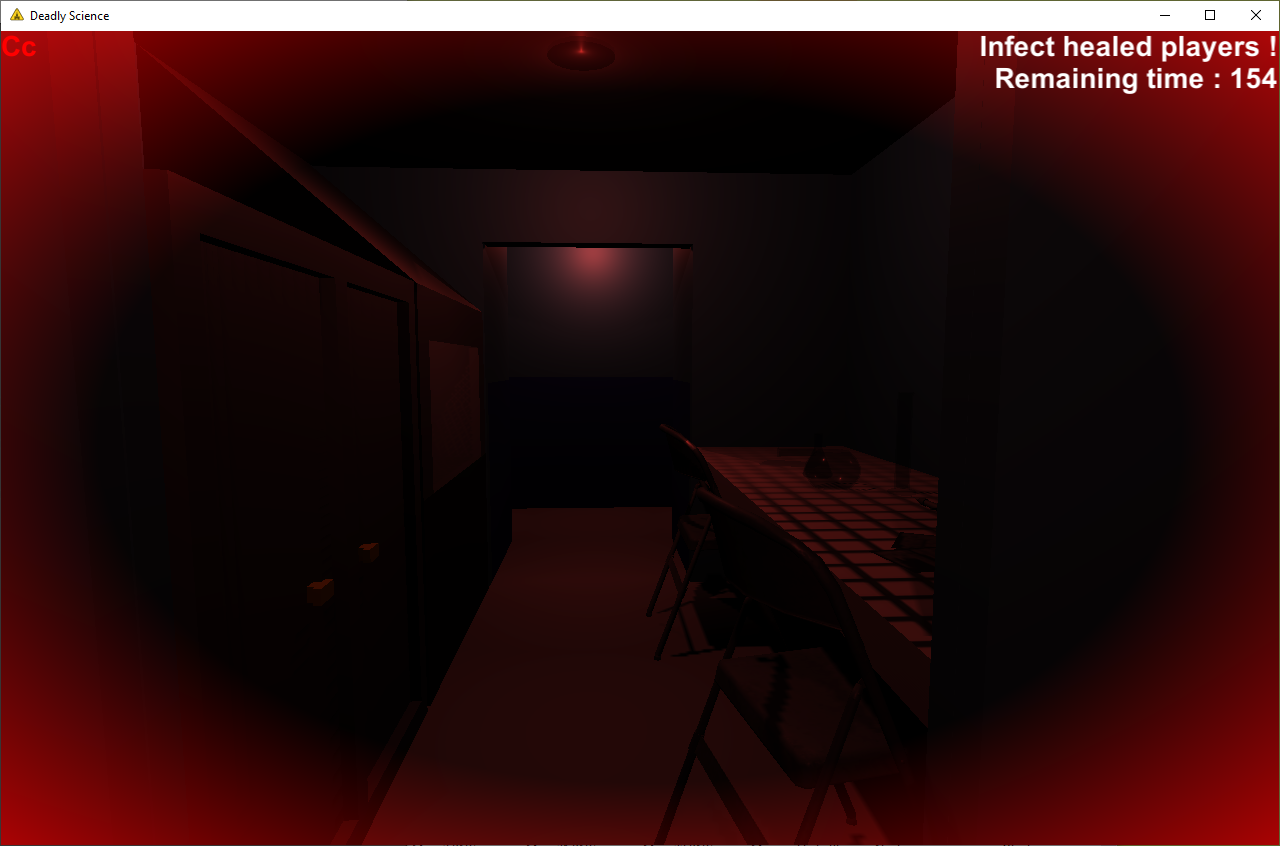
\includegraphics[width=0.8\textwidth]{cc/post_proc.png}
\caption{Une aura rouge sur la caméra d'un joueur condamné}
\label{cc_d}
\end{figure}


\newpage
\subsubsection{Joueur}


Le jeu est à jouer en réseau, le joueur a été implémenté en considérant qu'il doit être très modulable pour s'intégrer au réseau.
C'est pourquoi j'ai créé plusieurs modules qui peuvent s'enlever sous diverses conditions.
Voici les principaux modules :


\begin{itemize}
\item PlayerNetwork : Permets de gérer les événements liés au réseau et également
mets en place ou retire toutes les autres classes du joueur. Ce script est
toujours présent sur un joueur.
\item Player : Classe permettant de contrôler le joueur. Utilisée quand le joueur
est contrôlé par le client.
\item PlayerState : Classe gérant le statut du joueur. La classe est toujours
présente, ses attributs se font modifier seulement par le réseau.
\item PlayerMaster : Dispose de fonctions gérant le jeu et les phases. Ce module
est présent si le joueur est contrôlé par le client ainsi que le client est le
maître de jeu.
\end{itemize}


Il est important que chaque module d'un joueur soit coordonné avec les autres. Par exemple, si le réseau possède un problème et qu'un joueur se connecte en plusieurs secondes, il faut l'attendre, ensuite préparer le jeu (ce qui comprend la génération du labyrinthe) puis enfin lancer la première phase. PlayerNetwork est ainsi le chef d'orchestre qui va enlever certains modules au début du jeu. Il se charge également d'envoyer et de recevoir les événements liés au réseau.


Notre jeu tourne autour d'un système de statut, pour l'implémenter côté joueur j'ai fait appel au module PlayerState.
Pour décrire un statut, créer une énumération suffit. Un événement \emph{SetStatus} a été alors intégré à PlayerNetwork pour pouvoir le modifier en réseau.


Quand un joueur entre en collision avec un autre joueur, une fonction se charge de tester si les statuts peuvent se transmettre (dans le cas d'un joueur condamné par exemple) et l'événement réseau \emph{SetStatus} est lancé.


Vous avez sans doute remarqué que les joueurs possèdent des modèles 3D ainsi que des animations.
Nous avons préféré utiliser un modèle déjà fait sur l'Asset Store de Unity, car il est compliqué et surtout long de modéliser un humanoïde ainsi que de lui associer un squelette. Les animations aussi ont été trouvées sur l'Asset Store, néanmoins, nous avons nous même scripté les animations. En effet, nous utilisons le composant Animator de Unity qui permet de jouer des animations ainsi que de lancer des transitions entre deux animations. Pour ce faire, j'ai juste modifié des variables présentes dans l'animator à partir du script gérant les mouvements du joueur comme par exemple la variable \emph{onGround} qui est booléenne. Steve les a ensuite portés en réseau pour que chaque joueur puisse voir ses adversaires bouger correctement.


\paragraph{Physiques}


Comme dit précédemment, les mouvements du joueur ont un grand impact sur le gameplay, il est alors indispensable de bien gérer les physiques du joueur.
Pour ce faire, j'ai utilisé un composant nommé CharacterController. Le CharacterController remplace un RigidBody que peut porter un objet dans Unity. Il permet d'entièrement contrôler le joueur, c'est-à-dire que c'est le rôle du développeur de gérer les physiques comme les forces appliquées sur le corps. Le CharacterController prend juste en charge les collisions entre les autres objets pour ne pas passer au travers. Il est préférable d'utiliser ce composant, car nous pouvons par exemple enlever la gravité ou les forces de friction quand nous le voulons. Il est utilisé également pour éviter des bugs causés par le réseau, si deux joueurs sont au même endroit, il ne faut pas les éjecter.
Pour implémenter ceci, j'ai utilisé des règles simples de physique. C'est à dire que j'ai utilisé des variables comme la vitesse ou si le joueur était sur le sol pour savoir comment modifier la position de celui-ci.


\subsubsection{Endurance}


Parlons à présent du mécanisme d'endurance.
Cette fonctionnalité s'implémente en deux temps. Il faut premièrement détecter les coups entre joueurs puis gérer le mode assommé. Après cela, il faut tout porter en réseau et ceci comprend également l'affichage de la barre d'endurance au-dessus des joueurs. Pour détecter les coups, j'ai créé la fonction Player.Attack qui est appelée quand l'utilisateur clique. Cette fonction utilise des RayCasts fournis par Unity, ils décrivent une détection de collision par rayon. Il faut spécifier le point de départ du rayon, sa direction, sa distance ainsi qu'un masque qui permet de filtrer les collisions. Ce masque retient seulement la catégorie de joueur. Une fois touché, nous allons appeler un événement réseau qui va mettre à jour l'endurance voir le statut du joueur touché.
Pour le mode assommé, il suffit de mettre des conditions dans la fonction du joueur gérant ses mouvements.


Pour mettre tout cela en réseau, j'appelle une fonction tous les tiers de seconde qui synchronise les attributs comme l'endurance.
Elle n'est pas appelée plus souvent, car elle saturait le réseau ce qui avait pour effet de faire voler ou bien nager dans le sol les joueurs.


Un dernier élément ajouté est l'affichage de statut et d'endurance au-dessus de la tête des joueurs. Ces éléments appartiennent aux joueurs non contrôlés par le client et sont toujours tournés vers la caméra. Il faut alors enlever celui du client au début de la partie et les mettre à jour lors d'un changement de statut ou d'endurance.


\paragraph{Sérums}


Les sérums sont composés d'un modèle 3D le représentant, d'une boîte de collision pour être collecté ainsi qu'un script qui se charge d'avertir le jeu lors d'un sérum ramassé.
Un sérum peut être considéré comme un power up, car c'est un objet qui peut se faire collecter par un joueur, pour éviter de changer beaucoup de scripts après l'ajout des power ups, j'ai pensé à utiliser de la programmation orientée objet en créant une classe PowerUp qui est abstraite, elle possède une méthode OnCollect qui est appelée lors d'une collision avec un joueur, elle prend en paramètre le joueur et retourne si le power up doit être détruit. Il ne doit pas toujours se détruire, car un joueur ayant déjà collecté un sérum ne peut pas en prendre en autre. Le sérum utilise alors cette fonction dans sa propre classe.


\subsubsection{Audio}


Je me suis également occupé d'implémenter les sons et musiques au sein du jeu. Léandre s'est occupé de composer les musiques et pour ma part je les ai mixées et intégrées au jeu. Les éléments sonores composés sont l'intégralité des musiques ainsi que certains effets tels que ceux de victoire ou de défaite.
Les musiques et effets sont des listes regroupant à la fois un identifiant et un fichier audio. J'ai créé une classe Audio premièrement qui possède des fonctions statiques ainsi qu'une instance statique, je me suis inspiré du design pattern Singleton pour cette classe afin de rendre plus facile d'accès les méthodes. Cette classe doit être alors unique et pour cela j'ai fait appel à la fonction DontDestroyOnLoad de Unity, elle permet comme son nom l'indique de ne pas enlever l'objet ayant ce script lors d'un changement de scène. Les effets sonores et les musiques sont pour moi deux éléments distincts.

Les effets sonores sont des fichiers audio souvent de quelques secondes, ils interviennent lors de la victoire par exemple. Ces sons doivent se détruire automatiquement une fois terminés.

Quant aux musiques, elles ne se terminent jamais, elles se jouent en boucle et il n'y en a qu'une seule à la fois.

Avec Unity, ce n'est pas compliqué d'implémenter une fonction Play et SetMusic qui jouent soit un effet audio, soit de la musique. Le plus long a été de faire des transitions entre deux musiques.
Pour faire cela, j'ai utilisé un Animator, ce composant permet de gérer plusieurs animations sur un objet. Il y a deux animations : celle d'entrée et celle de sortie.

J'ai alors créé un autre script qui combine deux volumes, celui fournit par l'animation et celui des paramètres, comme leurs valeurs sont entre 0 et 1 il suffit de les multiplier entre elles pour obtenir le bon volume. Pour que les transitions se jouent au bon moment nous déclenchons un trigger dans l'animator, c'est juste une fonction qui déclenche une nouvelle animation. Ils se déclenchent au lancement de la musique et lors d'une transition. De plus, ces deux animations durent le même temps pour que ça soit plus agréable.




\newpage
\paragraph{Effets audio}


Lors de la seconde soutenance, j'avais introduit un mécanisme permettant de jouer des sons ainsi que des musiques comprenant des transitions. J'avais promis de rajouter quelques effets sonores, car il y en avait trop peu - chose promise, chose due - à présent, j'ai ajouté quelques sons tels que le son de victoire ou de défaite, le son de la prise d'un bonus ou même celui qui intervient lors d'un changement de phase. Je ne me suis pas seulement contenté d'ajouter de simples effets sonores, en effet, certains ont été un peu plus complexes à implémenter. Par exemple, le son des coups des joueurs, je voulais qu'on ait toujours une réponse à une action or lors d'un coup nous pouvons rater le joueur, comme le joueur ne se voit pas lui-même il ne peut pas voir si son coup a bien été pris en compte. De plus, il est illogique de jouer un son de coup réussi. J'ai alors cherché deux sons, un de coup réussi et un autre de coup raté, le bruit décrit un mouvement dans l'air. Il ne restait plus qu'à ajouter les conditions pour les lancer, je les ai mises dans la fonction Player.Attack lors du test de collision de joueur par rayons :


\begin{lstlisting}
si rayon touche joueur alors
	// Gestion du statut...
	jouer son "coup"
sinon
	jouer son "coup_rate"
fin
\end{lstlisting}


Un autre effet sonore qui demande un peu plus de temps à intégrer est l'effet de prise de sérum. Je voulais que les joueurs sachent quand quelqu'un prenait un sérum pour les presser un peu plus et rajouter du suspens. Il fallait là aussi ajouter deux sons distincts, celui joué au joueur qui prend le sérum et celui joué aux autres joueurs. Pour ce faire, j'ai voulu éviter d'ajouter des événements réseau et j'ai alors repris l'événement \emph{PlayerNetwork.OnSerum} qui est levé et envoyé dès qu'un joueur prend un sérum. Heureusement, j'avais déjà fait en sorte qu'il soit possible d'indentifier quel joueur prend ce sérum, il ne reste plus qu'à tester si ce joueur est le joueur contrôlé par le client puis nous savons quel son jouer.


\begin{lstlisting}
si joueur = joueur local alors
	jouer "serum"
sinon
	jouer "serum_long"
fin
\end{lstlisting}


\newpage
\subsubsection{Particules}


Les effets audio sont primordiaux pour un jeu, il y a aussi d'autres effets que nous pouvons ajouter pour améliorer notre jeu tels que les particules.
Les particules sont un ajout majeur de la dernière soutenance, elles permettent d'envoyer un signal de réponse aux actions du joueur. Elles donnent alors plus envie aux joueurs de s'attaquer entre eux ou de prendre des bonus.
À présent, les particules ont lieu lors d'un changement de statut ou lors d'un coup donné à un autre joueur. Elles sont assez simples, composées d'une image de point un peu flouté et parfois disposent de traînée colorée. Certaines propriétés sont animées comme la vitesse qui diminue plus la particule s'éloigne et aussi la couleur. La couleur est peu saturée au tout début, après 10 \% de son temps de vie, une couleur plus saturée, mais plus claire que la couleur principale apparait, elle laisse ensuite sa couleur principale qui s'assombrit en changeant un peu de teinte pour s'estomper.
J'ai la chance d'avoir déjà utilisé les systèmes de particules, c'est pour cela que cet ajout, bien qu'être important, a été simple et rapide à intégrer.


\paragraph{Systèmes de particules}


Pour manipuler des particules, il faut obligatoirement passer par un système de particules.
Il est très facile de comprendre pourquoi ceci est obligatoire. En effet, un système de particules est un objet qui va gérer les particules, c'est-à-dire qu'il va s'occuper de les faire apparaitre ou disparaitre et aussi va changer les propriétés des particules telles que leur couleur, taille, position... La raison pour laquelle un système est obligatoire est que les particules peuvent interagir entre elles et ont besoin d'un "chef d'orchestre" pour changer leurs propriétés.
Unity dispose d'un moteur de particules très poussé et complet, il n'est pas évident à utiliser au début, mais en s'habituant tout cela devient très vite simple. Il y a plusieurs catégories, vu que nos particules sont simples nous allons utiliser seulement les principales catégories.




%%% TODO : More space
\begin{center}
\emph{Lors de mes explications, je ne vais pas préciser les valeurs des propriétés, car il y a plusieurs systèmes de particules donc différentes valeurs}
\end{center}


\begin{figure}[H]
\centering
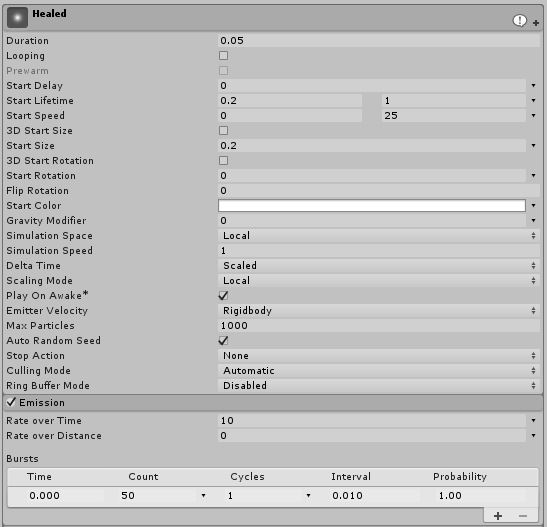
\includegraphics[width=0.8\textwidth]{cc/particles_main.png}
\caption{Les deux premières catégories}
\label{Les deux premières catégories}
\end{figure}


La catégorie principale permet d'ajuster la durée de vie ainsi que la vitesse de la particule. Pour que le système soit plus vivant je préfère utiliser des valeurs aléatoires entre certaines valeurs, cela évite notamment que les particules disparaissent d'un coup.


La seconde catégorie permet de modifier les propriétés d'émission de particules. Nous ne voulons pas ici qu'elles apparaissent en continu, mais qu'elles apparaissent d'un coup donc j'utilise le tableau \emph{Bursts} avec une entrée exécutée dès l'apparition du système.


\begin{figure}[H]
\centering
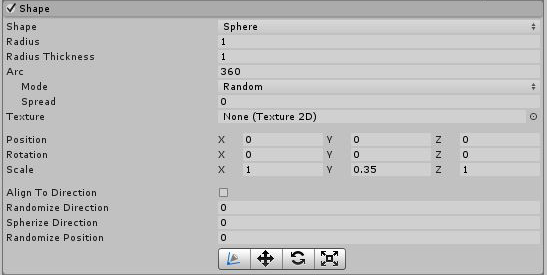
\includegraphics[width=0.8\textwidth]{cc/particles_shape.png}
\caption{Catégorie forme}
\label{Catégorie forme}
\end{figure}


La prochaine catégorie sert à modifier la forme d'émission. Les particules vont naître à l'intérieur de cette forme puis vont être expulsées en fonction des normales associées à la forme. J'ai utilisé uniquement des sphères que j'ai étirées pour avoir plus de particules sur l'axe horizontales que verticales, car nous ne regardons pas souvent en haut ou en bas donc cela permet de gérer moins de particules (elles peuvent être compliquées à gérer pour les ordinateurs peu puissants).


Deux autres catégories vont permettre de modifier la vélocité (c'est-à-dire la vitesse) ou la couleur en fonction du temps, on fournit des courbes qui vont faire évoluer des valeurs entre 0 et 1, la couleur est représentée par un dégradé, à gauche est la couleur quand la courbe donne une valeur proche de 0 et à droite quand la valeur est 1.


\begin{figure}[H]
\centering
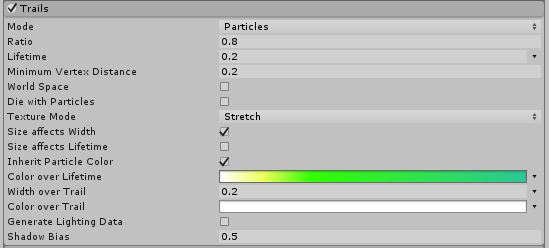
\includegraphics[width=0.8\textwidth]{cc/particles_trail.JPG}
\caption{Catégorie traînée}
\label{Catégorie traînée}
\end{figure}


Enfin, je vais parler de la catégorie se chargeant des traînées. J'ai fait en sorte qu'une certaine proportion des particules possède une traînée pour rendre plus joli. J'ai appliqué ici aussi un dégradé de couleur et modifié la largeur de traînée. Une autre option qui permet de rendre plus agréable l'effet est celle qui change le temps de vie en fonction de la durée de vie de la particule liée à cette traînée. Cela permet d'avoir une traînée dynamique, la fin de la traînée se rapproche de plus en plus du centre de la particule.


\paragraph{Gestionnaire de particules}


Maintenant que les systèmes de particules ont été créés, il va falloir s'intéresser à comment les gérer, c'est-à-dire comment les générer et détruire.
Un système de particule est rattaché à un simple objet pouvant être instancié, déplacé et même détruit. En pratique, le système de particules se détruit lui-même quand toutes les particules ont été générées.
Avant de commencer à coder la classe de ce gestionnaire, j'ai pensé qu'il ressemblait fortement au gestionnaire audio. En effet, il fournira une méthode statique principale qui fera apparaitre un système, tout comme la méthode \emph{Audio.Play} qui fait jouer un son (se qui revient à générer un objet avec un composant échantillon audio). Alors je me suis beaucoup inspiré de cette classe qui utilise notamment le design pattern du Singleton. Nous avons juste à mettre dans le menu une instance de ce gestionnaire puis lui dire de ne pas s'enlever lors du changement de scène. Ceci est très utile, car nous pouvons à partir de n'importe quel fichier instancié des particules, sans avoir besoin de posséder en attribut le gestionnaire.
Pour pouvoir regrouper les systèmes, j'ai utilisé un tableau composé de paires GameObject et String, le premier composant est le système de particules (une Prefab) et le second est l'identifiant de celui-ci. Pour remplir le tableau des systèmes, je préfère utiliser une nomenclature standardisée (comme pour Audio), tous les identifiants sont les mêmes que ceux des fichiers sans les extensions. Ils sont eux-mêmes nommés en snake case, c'est-à-dire en minuscule avec des underscores à la place des espaces. Je préfère utiliser une casse différente entre les fichiers sources et les fichiers de ressource.




\begin{lstlisting}
// Audio.cs
public static void Audio.Play(string id);


// Particles.cs
public static void Particles.Spawn(string id, Vector3 loc);
\end{lstlisting}


La méthode \emph{Particles.Spawn} prend en argument un identifiant qui est celui associé au système de particules ainsi qu'une position qui décrit l'endroit de création des particules. Une fois le tableau des échantillons rempli, nous avons juste à trouver le premier élément ayant cet identifiant. Après cela nous le clonons au bon emplacement et le tour est joué. Vous avez peut-être remarqué que nous ne pouvons pas changer la rotation, cela est normal, car les systèmes ont toujours la même rotation, orientée à la verticale et comme ils ont une forme de sphère allongée les autres axes de rotation n'influencent pas le système.


\paragraph{Types de particules}


J'ai brièvement annoncé quels étaient les types de systèmes de particules, je vais un peu approfondir la description de chaque type.


Commençons par les particules créées lors d'un changement de statut. Elles sont très semblables, seulement leurs couleurs et les conditions de création sont changées. Chaque statut a une couleur associée comme le violet pour les joueurs infectés, le vert pour les joueurs guéris et rouges pour ceux condamnés. Comme énoncé précédemment, c'est en fait un dégradé de couleur que j'associe aux particules et chaque dégradé a pour couleur principale, c'est-à-dire la plus saturée et la plus présente au cours de la vie de la particule, la couleur d'un statut. Ceci est valable aussi pour les traînées de ces particules. Quant à la création de ces systèmes, j'ai voulu que tous les joueurs puissent voir qu'un changement de statut a lieu, il a alors fallu mettre l'apparition des particules en réseau. Photon dispose d'une méthode \emph{Instantiate} qui permet de faire apparaitre un objet en réseau, je n'ai pas voulu utilisé cette méthode, car il faut après détruire l'objet avec la méthode de Photon \emph{Destroy} or les particules s'enlèvent automatiquement. Alors je suis allé dans le setter PlayerState.Status qui est appelé lors d'un changement de statut, peu importe le joueur, et en fonction du statut, j'instancie le bon système grâce à son identifiant. Au lieu de faire un switch, j'ai préféré utiliser un tableau où j'ai écrit chaque identifiant. Une énumération décrit seulement un type qui peut être considéré comme un entier non signé, j'ai alors pu convertir le statut en entier pour qu'il décrive l'indice de l'identifiant. Cette méthode est de complexité constante en temps ce qui est toujours mieux qu'un switch, mais je l'ai utilisée surtout pour rendre mon code plus joli et plus lisible, car les optimisations sont négligeables vu le faible nombre de statuts (il y en a seulement 4). Nous n'avons plus qu'à instancier les particules à l'endroit du joueur ayant changé de statut.


\begin{figure}[H]
\centering
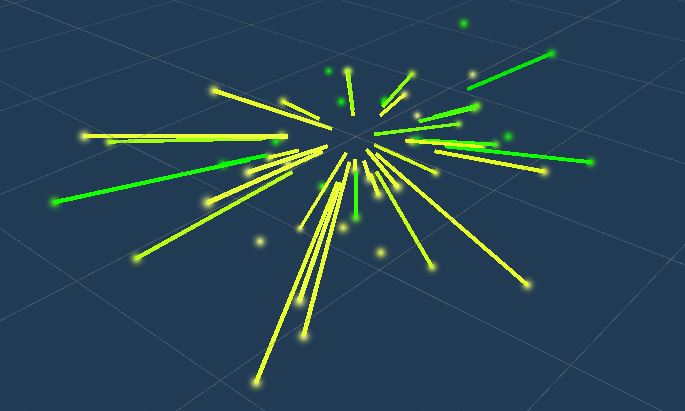
\includegraphics[width=0.8\textwidth]{cc/particles_healed.JPG}
\caption{Particules du statut guéri}
\label{Particules du status guéris}
\end{figure}




\begin{figure}[H]
\centering
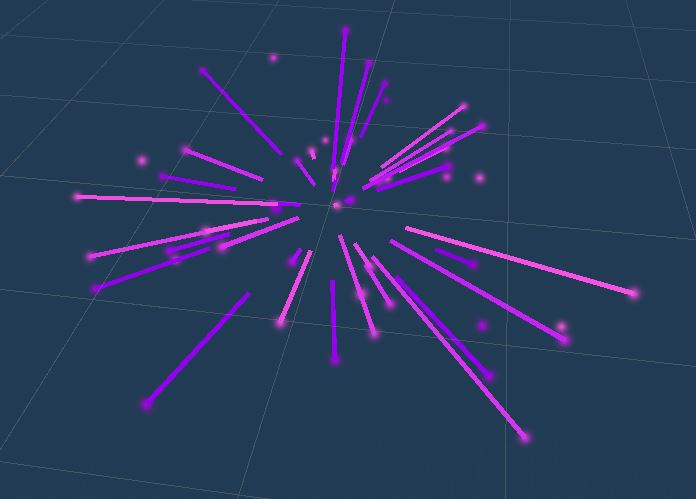
\includegraphics[width=0.8\textwidth]{cc/particles_infected.JPG}
\caption{Particules du statut infecté}
\label{Particules du status infécté}
\end{figure}




\begin{figure}[H]
\centering
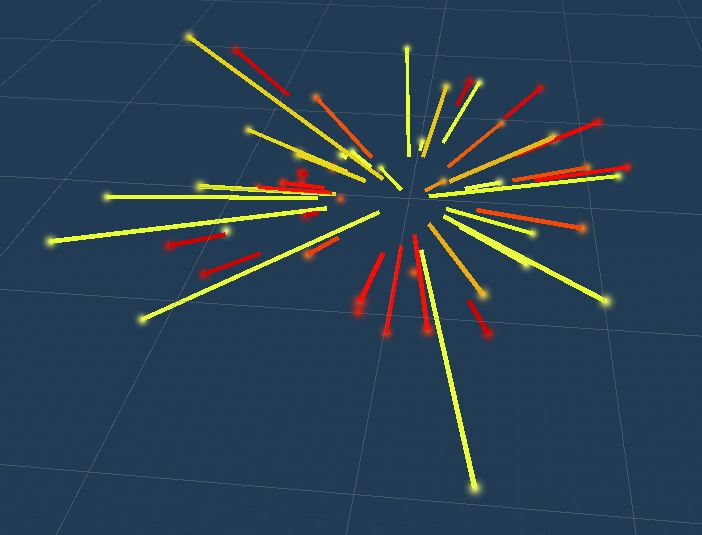
\includegraphics[width=0.8\textwidth]{cc/particles_revenge.JPG}
\caption{Particules du statut condamné}
\label{Particules du status condamné}
\end{figure}


Les particules associées aux coups sont des points rouges. Au début la couleur était blanche, mais nous ne les voyons pas assez donc je les ai passées au rouge. Pour ne pas les confondre avec celles de changement de statut en condamné, j'ai désactivé les traînées. C'est plus agréable sans traînées, car ces particules sont moins importantes que celles de changement de statut et interviennent plus souvent. Pour les instancier, il fallait les placer à l'endroit du coup et les crées seulement lors d'un coup réussi. Heureusement, j'ai pu utiliser le rayon fourni par le moteur physique de Unity, j'ai récupéré le rayon servant à détecter la collision entre les joueurs et pu retrouver la position du coup comme je détecte au maximum un seul obstacle.


\begin{figure}[H]
\centering
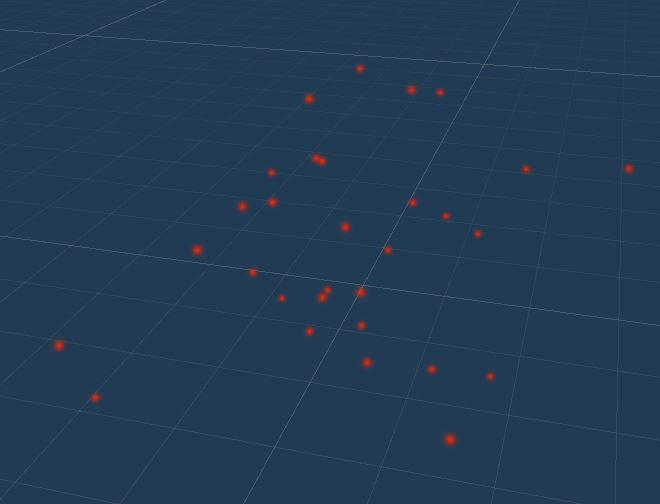
\includegraphics[width=0.8\textwidth]{cc/particles_hit.JPG}
\caption{Particules de coups}
\label{Particules de coups}
\end{figure}



\newpage
\paragraph{Effets visuels supplémentaires}


Je vais à présent parler du contenu qui m'a fait le plus plaisir à implémenter du projet, le post-traitement d'image. J'entends par ceci l'effet vignettage rouge animé que nous voyons quand nous sommes condamnés. Cet effet immerge le joueur dans la peau du personnage et permet d'augmenter le sentiment de panique que fait face un joueur encore infecté en seconde phase. Cet effet visuel a lieu seulement sur l'image générée par la caméra, les différents éléments d'interface utilisateur ne sont alors pas affectés par celui-ci.
Pour implémenter ceci, j'ai utilisé les shaders de Unity. Cet effet était un peu nouveau pour moi, car je n'avais jamais utilisé ces techniques dans Unity même si j'avais déjà utilisé Open GL et ses shaders donc je savais à peu près comment m'y prendre. Le langage des shaders quant à lui est proche du C que j'utilise régulièrement. Un shader est un programme exécuté par le GPU et permet en général de modifier les propriétés de chaque sommet des triangles dessinés ou de modifier les pixels qui les composent. Je ne vais utiliser seulement les fragment shaders ici, c'est-à-dire les shaders de modification de pixels.
Avant de coder quoi que ce soit, il faut bien évidemment penser à ce que l'on veut avoir comme résultat.
Nous voulons un dégradé radial partant du centre et s'estompant aux coins de l'écran. La couleur du dégradé est rouge, j'ai pensé à ajouter à la couche d'un pixel déjà présent une certaine dose de rouge au lieu de remplacer cette valeur par une nouvelle. Ce dégradé ne s'étend pas exactement du centre de l'écran à ces coins, j'ai voulu pouvoir régler à partir de quelle proportion de l'écran celui-ci commence, et aussi quand il se finit afin de pouvoir ajouter une animation faisant penser à un battement de coeur. Dernièrement, je voulais une valeur de force de l'effet, elle est comprise entre 0 et 1 et permet d'ajuster la transparence du dégradé.
Après avoir pensé au résultat que nous voulons obtenir, il faut penser à comment implémenter l'effet. J'utilise de simples formules d'algèbre ou de géométrie. De plus, chaque pixel envoyé au programme a une position en coordonnées UV, donc chaque valeur est entre 0 et 1. Ceci est très pratique pour trouver le centre de l'écran qui est juste à la position (0.5, 0.5).
Commençons par trouver un vecteur partant du pixel à modifier jusqu'au centre de l'écran.


\begin{lstlisting}
// i est le pixel
float2 position = (i.uv - .5) * 2;
\end{lstlisting}


Cette variable va servir à trouver la distance au centre du pixel. Seulement, je voudrais une position normalisée, c'est-à-dire comprise entre 0 (le point est au centre) et 1 (le point est sur un des quatre coins). Comme nous sommes en coordonnées UV, une diagonale possède une longueur de $\sqrt{2}$.
Nous pouvons mettre à l'échelle le vecteur position en doublant sa longueur pour avoir une distance maximale de $\sqrt{2}$ puis diviser par $\sqrt{2}$ le résultat.


\begin{lstlisting}
float dist = sqrt(position.x * position.x + position.y * position.y) / 1.41f;
\end{lstlisting}


Il reste une dernière transformation à appliquer pour prendre en compte l'animation.
J'ai alors ajouté la constante \emph{HEART\_POS} et aussi une autre \emph{HEART\_STRENGTH} ainsi qu'une variable \emph{\_AnimRatio} que nous mettrons par la suite à jour dans notre script.

On obtient ainsi cette ligne de code :


\begin{lstlisting}
float dist = (sqrt(position.x * position.x + position.y * position.y) / 1.41f - _AnimRatio * HEART_POS) * (1.f - _AnimRatio * HEART_STRENGTH);
\end{lstlisting}


Ajoutons maintenant une fonction qui change la valeur entre 0 et 1 en fonction des constantes \emph{MAX\_DIST} et \emph{MIN\_DIST} :


\begin{lstlisting}
float map(float dist)
{
	float range = MAX_DIST - MIN_DIST;


	dist -= MIN_DIST;
	dist /= range;


	return clamp(dist, 0, 1);
}
\end{lstlisting}


Maintenant il ne reste plus qu'à modifier la couleur du pixel :


\begin{lstlisting}
col.r += map(dist) * STRENGTH;
\end{lstlisting}


Notre shader est presque opérationnel, il faut l'ajouter sur la caméra en créant un matériau et donnant ce shader à celui-ci puis intégrer l'animation. L'animation est très simple, c'est juste une sinusoïde qui est comprise entre 0 et 1, la période de celle-ci peut être modifiée à partir de Unity. Pour l'implémenter, nous avons besoin juste d'une variable de temps puis nous calculons la valeur que prends cette sinusoïde en cette abscisse puis l'envoyons au GPU :


\begin{lstlisting}
// PlayerCam.LateUpdate
time += Time.deltaTime * heartSpeed;
postFx.SetFloat("_AnimRatio", .5f + Mathf.Sin(time) * .5f);
\end{lstlisting}


En changeant un peu les constantes, nous arrivons à un résultat très satisfaisant.


\newpage
\paragraph{Finalisation du jeu}


Après les divers effets ajoutés, nous avons pu tester et apprécié notre jeu. Il manquait quelques finitions à apporter.
Nous avons premièrement remarqué qu'un joueur peut être désavantagé s'il possède une mauvaise connexion ou que son jeu met du temps à charger. En effet, les joueurs ayant de meilleures connexions peuvent commencer à chercher les sérums en avance. Pour régler ce problème, j'ai désactivé les mises à jour des joueurs dans certaines conditions comme au début de la partie, à la fin et en pause, à noter que les deux derniers sont purement esthétiques. Désactiver la mise à jour du joueur comprends les physiques vu que les joueurs ne répondent pas aux physiques de Unity, mais à celles j'avais créées avant la première soutenance et comprends également toutes les actions et mouvements que font les joueurs, car les entrées sont ignorées (seulement celles liées au jeu ne le sont pas comme la pause).

Un autre aspect modifié est le label au-dessus de la tête du joueur. Il y avait marqué player or nous avons à présent implémenté des noms personnalisés. Pour changer le nom, il suffit de récupérer l'identifiant du joueur instanciant l'objet Player puis changer la propriété text du label.

Dernièrement, d'autres modifications mineures ont été ajoutées comme le changement de taille des boîtes de collisions des joueurs et des sérums et aussi la désactivation des attaques de joueurs quand ils sont assommés.


\paragraph{Résultats}


Pour conclure sur mes modifications apportées depuis la dernière soutenance, je trouve que le cahier des charges a été correctement respecté, aucun élément n'a été oublié ni incorrectement implémenté, au contraire, il y a eu même plusieurs ajouts supplémentaires.


J'ai beaucoup apprécié faire partie de cette équipe ainsi que d'avoir participé à ce projet, j'ai appris à travailler en groupe sur un long projet et également approfondi certaines connaissances ou maîtrises d'outils comme git par exemple que j'utilisais trop peu avant.

%%%%%%%%%%%%%%%%%%%%%% Leandre %%%%%%%%%%%%%%%%%%%%%%%%%%%%%%%%%%%%%%%%%%%%%%%%%%%%%%%%%%%%%%%%%%%%%%%%%%%%%%%%%%
\subsection{Léandre}
\newpage
\subsubsection{Labyrinthe}

\paragraph{Génération aléatoire du Labyrinthe}
Au début du projet, il a été décidé que je serais le responsable de l'ensemble des éléments aléatoires du jeu, ainsi que de la direction artistique. J'ai ainsi commencé en mettant au point un algorithme permettant de générer un dédale de telle sorte que l'ensemble des salles soit accessibles, et que pour accéder à une salle à partir d'un endroit du labyrinthe, il y ait plusieurs itinéraires. L'algorithme a été développé en faisant en sorte qu'il n'y ait aucune sortie, et que l'on puisse modifier la taille du labyrinthe. Au final, l'algorithme correspond à peu de choses près à l'algorithme de Prim, excepté le fait que le nombre d'impasse est nettement moins important. A côté de cette fonction, j'ai également créé une seconde fonction retournant une liste d'entiers aléatoires distincts dans un intervalle donné.

\paragraph{Labyrinthe en Cubes}
A partir de cet algorithme, on obtient donc une liste dont les valeurs correspondent directement aux passages de chaque "case" du labyrinthe. Pour vérifier que l'algorithme fonctionnait bien, et vite, j'ai mis au point une petite fonction qui se charge d'afficher la carte du labyrinthe ainsi formé dans une console. Après de nombreux tests, aucours desquels j'ai modifié la taille du dédale pour obtenir des configurations rectangulaires, cubiques, voire linéaires pour vérifier le bon fonctionnement de l'algorithme, j'ai transposé le tout sur Unity. J'ai alors modifié la fonction d'affichage en faisant en sorte qu'à la place de mettre des caractères dans une console, Unity instancie des cubes dans une "Scène" prévue à cet effet.

\begin{figure}[H]
    \centering
    
\includegraphics[width=0.8\textwidth]{Blocs.png}
    \caption{La toute première version du labyrinthe}
    \label{La toute première version du labyrinthe}
\end{figure}

\paragraph{Labyrinthe en Salles}
Ensuite, étant donné que nous souhaitions donner à l'ensemble une structure évoquant plus un laboratoire souterrain qu'un jeu de cube pour enfants, j'ai développé une autre fonction pour afficher non pas les murs séparément, mais directement des modèles 3D de salles avec les passages, pour simuler un vrai labyrinthe. La difficulté était ici de bien configurer pour chaque salle l'orientation, ainsi que la position au sein du labyrinthe. Mais j'ai tout de même conservé l'affichage en bloc en vue d'autres tests de génération de l'algorithme, étant donné que cet affichage permet de vérifier plus aisément que la carte du labyrinthe soit valable. Les modèles 3D que j'ai utilisé étaient surtout là pour simuler la carte dans un labyrinthe, et pour effectuer des tests en multijoueur.

\begin{figure}[H]
    \centering
    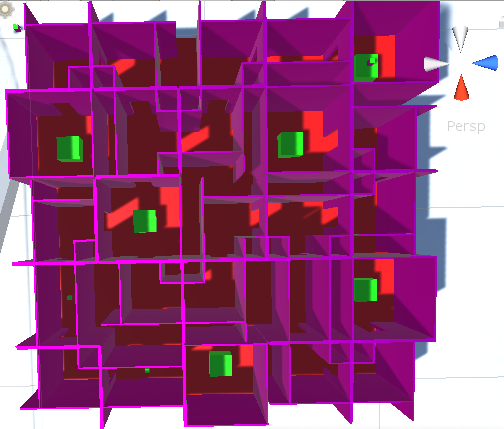
\includegraphics[width=0.8\textwidth]{Salles.png}
    \caption{La deuxième version du labyrinthe}
    \label{La deuxième version du labyrinthe}
\end{figure}

\paragraph{Labyrinthe et Sérums}
A partir de là, on obtient donc un labyrinthe correct, bien que dénué de décorations évoquant un laboratoire. Mais bien qu'il y ait un format correct, ce n'était pas encore jouable : il manquait bien sûr les Sérums et les Joueurs. Concernant les Joueurs, Célian a implémenté une rampe permettant de monter pour sauter directement dans le complexe. En revanche pour les sérums, il nous fallait prendre en compte plusieurs facteurs. Premièrement, un Sérum ne devait pas être implémenté à l'intérieur d'un autre Sérum. Deuxièmement, un Joueur ne devait pas être instancié au même emplacement qu'un Sérum, pour éviter qu'un Joueur ne se retrouve infecté dès le début de la partie. Pour cela, j'ai réutilisé la fonction permettant d'obtenir une liste d'entiers aléatoires distincts. Avec cette fonction, il m'était en effet possible d'isoler sept "cases" du complexe dans lesquelles seraient respectivement implémentés les quatres joueurs et les trois sérums. Ainsi, au lancement du jeu, j'ai fait en sorte que le joueur génère les sérums à l'emplacement souhaité. Pour les Sérums, nous n'avions alors que des cubes mauves pour les représenter. 

\paragraph{Labyrinthe en Réseau}
Restait alors la question de l'initialisation du labyrinthe en réseau. La difficulté était alors de faire en sorte que chaque joueur ait la même carte, et que les Sérums réagissent en réseau. Concernant ce second point, il nous est apparu nécessaire que les sérums, ainsi que les positions des joueurs et la carte du dédale, soient générés par un seul joueur. Le Joueur le plus reconnaissable en réseau étant le Créateur de la Partie, j'ai donc rajouté une condition à la génération du labyrinthe pour faire en sorte que le Créateur du Salon soit le seul à être en mesure de construire le labyrinthe, en instanciant des objets Photon en réseau. Le processus marchait bien pour la génération avec l'affichage en blocs, pour les murs et les Sérums. Mais nous avons rencontré quelques difficultés avec l'affichage en salles. En effet, dans la Partie du Créateur de la Partie, tout se générait correctement. Mais concernant les autres joueurs, nous nous sommes vite rendus compte que les salles étaient toujours orientées dans le même sens. Ce n'est qu'après coup que nous avons réalisé que le problème venait du fait que Photon n'enregistrait pas les rotations de salles effectuées par le Créateur du Salon. Nous avons rapidement corrigé ce détail, et après cela, nous avons pu commencer à effectuer des semblants de partie dans le labyrinthe, même si la seconde phase ne se lançait pas encore.

\paragraph{Répartion des Joueurs}
Le prochain objectif concernant la génération de la partie était alors de faire en sorte que les Joueurs apparaissent à des endroits différents dans le labyrinthe. Avant de commencer à nous attaquer directement à l'aléatoire, nous avons décidé de faire en sorte que les joueurs apparaissent sur quatre socles à l'extérieur du dédale. Après de nombreux essais, Steve a remarqué que via Photon, les Joueurs n'apparaissaient pas tous en même temps, mais les uns après les autres. Il s'est alors appuyé sur ce détail pour distinguer les Joueurs avec leur arrivée dans la Partie, en prenant en compte le nombre de Joueurs déjà présents. Effectivement, grâce à ce procédé, nous avons réussi à faire en sorte que les joueurs ne puissent pas apparaître au même endroit. Mais en utilisant cette méthode avec les quatres entiers prédéfinis pour les positions des joueurs dans le labyrinthe, nous nous sommes très vite rendus compte qu'il y avait une faille dans notre procédé. En effet, rien ne garantissait que le Master soit instancié en premier, ce qui faisait que souvent, les joueurs qui avaient le malheur d'apparaître avant lui se retrouvaient les genoux dans le sol. Steve a alors rajouté une option permettant de faire en sorte que le Créateur de la Partie soit le premier Joueur à être instancié, et envoit un message aux autres joueurs pour qu'ils puissent le rejoindre dans le labyrinthe. A partir de là, nous avons pu commencer à simuler de véritables débuts de partie.

\paragraph{Un décor de laboratoire}
Avec Yann, nous nous sommes alors appliqué à donner à l'ensemble un aspect beaucoup plus agréable que les modèles 3D rose vif et vert clair que nous utilisions. Nous nous sommes donc intéressé à Blender. J'ai commencé par créer un modèle pour les Sérums plus digne d'un véritable laboratoire qu'un bête cube tout droit sorti d'une caisse de jouets pour enfants. Puis nous nous sommes concentrés sur les salles. Nous avons commencé par déterminer les différents types de salle que l'on peut croiser dans un laboratoire : des salles de stockage, des salles d'information, des salles d'expérimentation, des couloirs, des salles de réflexion et des serres. Nous avons ensuite réparti ces catégories de salles en fonction de la probabilité d'avoir un certain nombre de portes, afin de les rétablir équitablement entre les différentes salles du labyrinthe. Ainsi, les salles de stockage n'ont qu'une porte et forment des impasses, les salles d'information en ont quatre et correspondent à des croisements, les salles d'expérimentations en ont deux et forment respectivement un couloir droit et un couloir tournant, et les couloirs classques et les salles de réflexion, elles ont trois portes, il s'agit donc d'embranchements.

\begin{figure}[H]
    \centering
    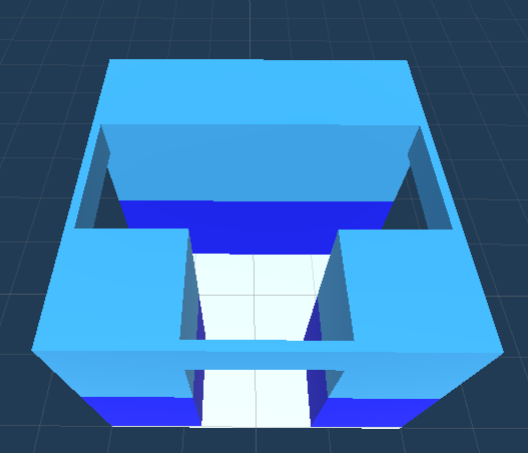
\includegraphics[width=0.8\textwidth]{Bifurc.png}
    \caption{Une des deux intersections dans le dédale}
    \label{Une des deux intersections dans le dédale}
\end{figure}

\paragraph{De nouveaux modèles 3D}
Je me suis ainsi occupé des serres, des salles d'expérimentation et des couloirs, tandis que Yann s'occupait des salles de réflexion, des salles d'information et des salles de stockage. Nous avons ainsi produit des modèles 3D à partir de Blender, que nous avons ensuite inséré à la place des modèles roses des précédentes version du labyrinthe. Nous avons fait attention à ce que les portes n'aient pas de rebords bloquants, afin de permettre aux Joueurs de courir plus aisément à l'intérieur du dédale. Cependant, nous avons eu un problème avec les salles d'information ; en effet, à la base, Yann avait prévu de mettre quatre écrans reliés avec un câble pendant du plafond. Le problème se posait pour les Joueurs et pour les Sérums : si un Sérum apparaissait dans ce type de salle, les écrans le rendaient inaccessible. De même, un joueur apparaissant dans cette salle se retrouvait bloqué par le câble au plafond, étant donné que les Joueurs arrivent du dessus du dédale. Nous avons donc modifié la configuration de manière à laisser l'accès libre au centre de la pièce. A côté de ça, il restait encore trois détails à régler pour la génération complète du labyrinthe : le mobilier, les salles d'attente où apparaissent dans un premier temps les Joueurs, et les lumières.


\begin{figure}[H]
    \centering
    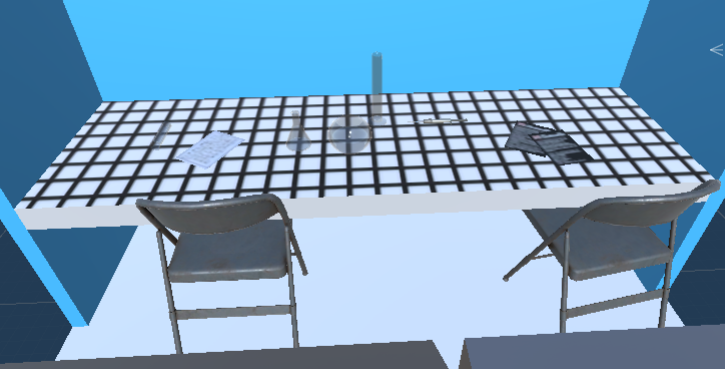
\includegraphics[width=0.8\textwidth]{labo2.png}
    \caption{Une paillasse pour des expériences}
    \label{Une paillasse pour des expériences}
\end{figure}

\begin{figure}[H]
    \centering
    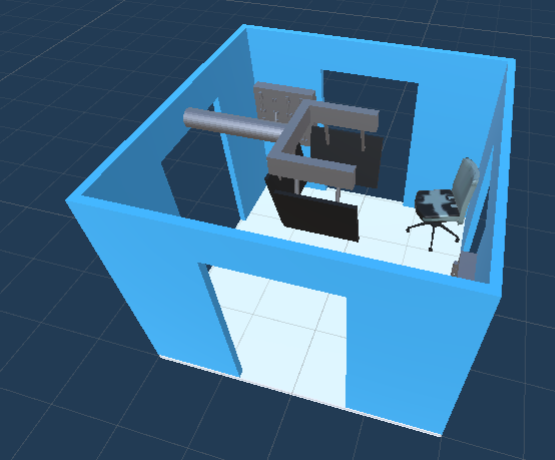
\includegraphics[width=0.8\textwidth]{Carrefour.png}
    \caption{Une salle pour transmettre les informations.}
    \label{Une salle pour transmettre les informations.}
\end{figure}

\paragraph{Luminosité}
Concernant le mobilier, je me suis appliqué à mettre des chaises, des ustensiles, des fioles, des plantes et des feuilles dans les modèles 3D, afin de donner l'impression qu'il s'agisse d'un véritable lieu de travail. De plus, je me suis amusé à glisser des références à d'autre jeux dans le décor. Peut-être aurez-vous l'occasion de les découvrir ? Mais qu'importe. Pour les salles d'attente, j'ai préféré faire en sorte que chaque joueur initialise sa propre salle en réseau, plutôt que de laisser au Créateur de la Partie le soin de tout charger. La décoration de ces salles est nulle, il s'agit juste de dissimuler l'extérieur du labyrinthe en attendant que tout les joueurs soient instanciés, afin de les faire commencer en même temps. Le seul élément distinctif est un trou dans le sol, qui permet de faire tomber le Joueur dans les méandres du dédale des souterrains du laboratoire. Enfin, concernant les lumières, j'ai créé un autre modèle 3D, un plafond, avec une lampe. La couleur de cette lampe est modulable directement via une fonction, ce qui permet entre autre de modifier sa couleur. Afin d'assurer le meilleur rendu possible, nous avons décidé de mettre les lumières en qualité importante, afin d'éviter les problèmes d'ombres entre les différents éléments du dédale. J'ai également prit soin de surélever le plafond si la salle était destinée à accueillir un Joueur. Enfin, j'ai annulé la luminosité ambiante de la Scène Unity. 


\begin{figure}[H]
    \centering
    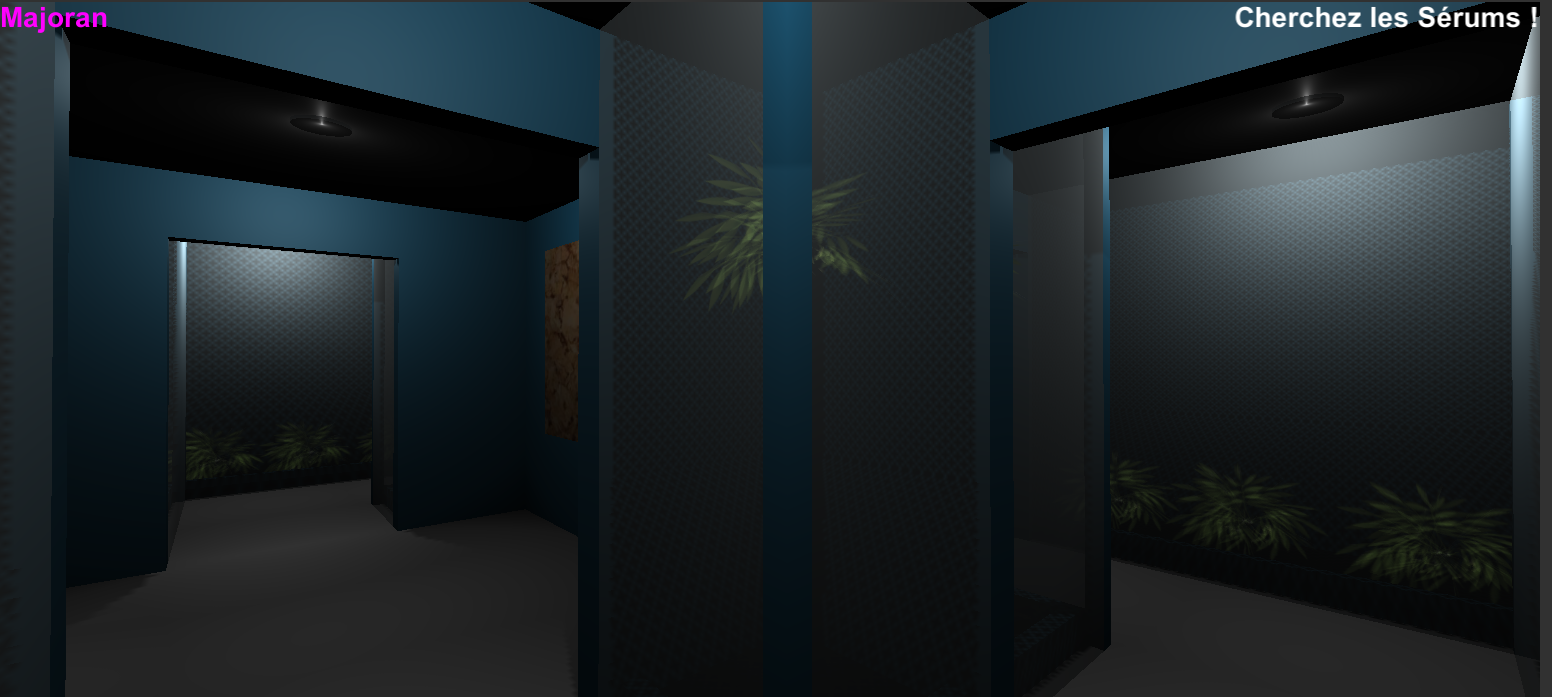
\includegraphics[width=0.8\textwidth]{Lumieres.png}
    \caption{Le rendu semble plus réaliste ainsi.}
    \label{Le rendu semble plus réaliste ainsi.}
\end{figure}

\paragraph{Mode Nocturne}
Le rendu est beaucoup plus réaliste que ce que nous avions précédemment. Cela dit, les lumières sont coûteuses en puissance. Pour éviter des problèmes avec Photon, nous avons décidé de limiter le nombre de salles possibles dans un labyrinthe à seulement 400. De plus, j'ai eu l'idée d'implémenter un second mode de jeu. Il s'agit du mode "NOCTURNE". Comme son nom l'indique, ce mode permet au Joueur de se retrouver dans un labyrinthe plongé dans le noir. L'unique lumière venant alors des joueurs, ce mode peut changer la donne, puisqu'il devient dès lors très difficile de se cacher. De même, à moins qu'il n'y ait un joueur devant soi, il est très dur de deviner les salles se trouvant devant le joueur actuel, ou même s'il y a un Sérum devant soi. Ce mode est donc beaucoup plus plaisant à jouer, non seulement pour l'ambiance beaucoup plus prenante que dans le mode "CLASSIQUE", mais également parce que les éventuels ralentissements dûs à un effort de l'ordinateur pour les lumières ne sont plus du tout présents. Un autre détail concernant les lumières est que j'ai fait en sorte que lorsque l'on passe en seconde phase et que l'on est en mode "CLASSIQUE", les lumières des lampes, jusque là blanches, deviennent rouges, afin d'évoquer de manière plus concrète une alarme de laboratoire.

\begin{figure}[H]
    \centering
    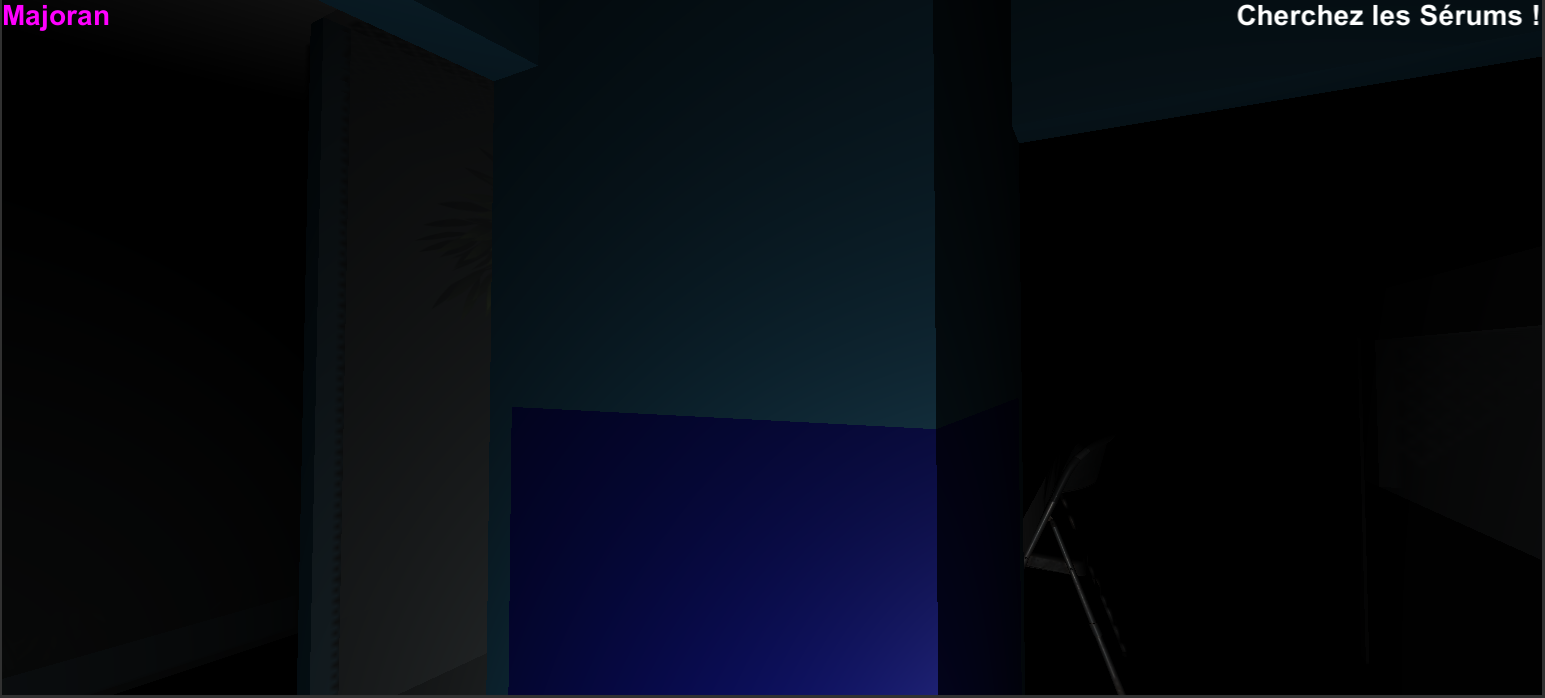
\includegraphics[width=0.8\textwidth]{Nocturne.png}
    \caption{Y a-t-il un sérum devant vous ? Ou une impasse ? Mystère...}
    \label{Y a-t-il un sérum devant vous ? Ou une impasse ? Mystère...}
\end{figure}

\subsubsection{Musiques}
\paragraph{Première tentative}
Pour travailler sur les musiques du jeu, j'ai utilisé un logiciel de partition nommé MuseScore, qui, en plus d'être gratuit, permet de générer directement une partition complète avec de nombreux instruments, et d'exporter la piste sonore en fichier MIDI. J'ai commencé dans un premier temps à faire plusieurs essais d'ambiance pour le thème de la Recherche de Sérum. Je tenais à rendre l'atmosphère assez stressante. Pour cela, j'ai utilisé un violon qui émet une note à intervalles précis et réguliers, à la manière d'une alarme d'évacuation. J'ai ensuite rajouté une percussion pour renforcer l'ambiance pesante et lourde, tout comme la contrebasse qui se charge du thème. Ensuite, Célian a remixé la piste obtenue, et le résultat est celui que vous pouvez entendre à vos oreilles en lançant une nouvelle partie.

\paragraph{Autres thèmes}
Ensuite, j'ai commencé à faire le thème du Menu Principal. Ici, je tenais à rendre l'atmosphère plutôt pesante et inquiétante. J'ai donc inséré en fond un piano qui répète la même note à la manière d'un tictac d'horloge, accompagné d'un trombone qui se charge de la basse. Enfin, j'ai également composé deux mélodies, l'une pour la victoire, la seconde pour la mort du joueur. Pour la première, j'ai cherché à faire quelque chose d'assez joyeux et léger, tandis que pour l'autre, j'ai utilisé des instruments beaucoup plus graves ainsi que des notes plus longues pour accentuer le sentiment de deuil. Tout comme pour la musique de la recherche de sérums, c'est Célian qui s'est chargé de remixer le tout, en modifiant notamment l'instrumentation. Actuellement, le jeu possède donc quelques musiques originales. Le problème, c'est que... Ce n'est pas dit que beaucoup de personnes apprécient. Mais au moins, il n'y aura pas de soucis avec les droits d'auteurs !

\subsubsection{Objets}
\paragraph{Génération d'Objets}
Etant donné que nous étions en avance sur nos prévisions de progression dans le projet, nous nous étions dis lors de la seconde soutenance que nous aurions peut-être le temps de rajouter quelques éléments qui ne figuraient pas dans le cahier des charges avant la dernière soutenance. C'est effectivement ce qu'il s'est passé. Nous avons donc décidé d'implémenter un système d'Objets récupérables au sein des laboratoires, afin d'aider les Joueurs ou, au contraire, de les gêner. Pour cela, j'ai tout d'abord réfléchi à l'implémentation des Objets. Un Objet doit remplir plusieurs critères. Premièrement, il ne doit jamais apparaître à l'intérieur d'un Sérum. Ensuite, il ne doit pas y avoir d'Objets à chaque salle du Labyrinthe. Pour ces deux raisons, nous ne pouvions pas mettre au point un système d'apparition d'Objets à intervalle de temps réguliers, car dans le cas où les Joueurs auraient peur des éventuels effets négatifs, le nombre d'Objets ne cesserait d'augmenter jusqu'à dépasser la contenance du labyrinthe, ce qui n'est absolument pas le but recherché. Finalement, nous avons décidé de faire en sorte que dans le Labyrinthe, il y aurait chaque fois un nombre constant d'Objets, Sérums compris. Ainsi, lorsqu'un Objet ou un Sérum est ramassé, il suffit juste d'évaluer une case ou un Sérum ou un autre Objet ne se trouve pas, et d'y générer le nouvel Objet. Ce système permet ainsi d'éviter un surplus d'Objet dans le labyrinthe, et de rendre la recherche des Objets relativement dynamique, puisqu'ils ont la possibilité de se renouveler à l'infini sans pour autant menacer la fluidité du jeu. 

\paragraph{Nombre d'Objets}
Au début de la partie, nous devons donc définir un nombre d'Objets de base. Il fallait bien sûr prendre en compte le nombre de Sérums nécessaires, mais également la taille du labyrinthe. En effet, dans un labyrinthe 20x20, s'il n'y a que trois Objets, en trouver relève du défi pur et dur. Nous avons donc choisi de faire en sorte qu'il y ait toujours un Objet par lot de 25 salles. Ainsi, un labyrinthe 10x10 aura quatre Objets, tandis qu'un labyrinthe 20x20 en comportera seize, ce qui est raisonnable étant donné qu'un dédale 20x20 est quatre fois plus grand qu'un dédale 10x10. De plus, j'ai pris soin de vérifier que pour le nombre, il y avait assez pour mettre suffisamment de Sérum au début de la partie. Si le nombre de salles est trop faible, j'augmente donc le nombre d'Objets pour qu'il y ait au moins le bon nombre de Sérums au début. Concernant l'apparence des Objets, vous aurez peut-être reconnu les cubes de Portal.

\begin{figure}[H]
    \centering
    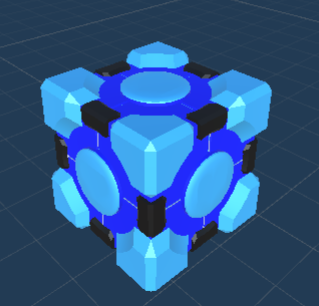
\includegraphics[width=0.8\textwidth]{Objet.png}
    \caption{Un Objet}
    \label{Un Objet}
\end{figure}

\paragraph{Sélection d'Objet}
Maintenant que les Objets sont implémentés, il faut leur ajouter des effets différents. Actuellement, il existe une douzaine d'effets différents. Il existe trois catégories d'effets, et deux sortes d'Objets. Les catégories sont : effets positifs, effets négatifs, et effets inutiles. Les Objets, eux, peuvent soit s'appliquer au moment où le Joueur les prend, soit rester sur le Joueur jusqu'à pouvoir être utilisés. Pour ces derniers, j'ai donc rajouté un tableau de booléens visant à déterminer si le Joueur a déjà les effets d'un Objet spécifique, et surtout d'afficher la liste de ces Objets sur son écran. Bien sûr, un Joueur ne peut pas récupérer un Objet qu'il a déjà. L'algorithme que j'ai utilisé choisit donc un des Objets parmi ceux que le Joueur peut potentiellement recevoir. Par exemple, si le Joueur est déjà équipé de Bottes de Pégase, il ne peut pas retomber sur des Bottes de Pégase à moins de les avoir perdues. De plus, certains Objets nécessitent de se trouver en seconde phase, et d'autres ne peuvent être pris que par un Joueur Guéri.

\paragraph{Image de la Carte}
Avant de commencer à faire de nombreux Objets, j'ai commencé par développer la Carte. En effet, j'avais pris soin de laisser le coin inférieur-gauche de l'écran en vue de cet Objet. Le problème, c'est qu'il n'y a qu'un seul joueur qui a accès au plan du Labyrinthe. Le Créateur de la Partie. J'ai donc réarrangé mon algorithme de construction de la carte. En effet, j'avais, lors de mes recherches pour la construction du labyrinthe, formulé deux versions : une par salle, qui est d'ailleurs utilisée pour générer le labyrinthe tel que vous le voyez maintenant, et une par bloc, qui permettait justement de comparer les plans des différents labyrinthes de manière très simple. Tout ce qu'il me restait à faire, c'était donc de transposer ces deux algorithmes pour construire à la fois le labyrinthe tridimensionnel et l'image renfermant la carte du labyrinthe. Ensuite, Steve et Célian se sont débrouillés pour faire en sorte que lorsque le Créateur du Salon envoie le message aux autres joueurs leur indiquant qu'ils peuvent générer leur personnage, il leur envoie également le Mode de jeu actuel, les dimensions du Labyrinthe, et la carte. Voici comment j'ai pu faire en sorte que tous les Joueurs aient accès à la Carte.

\begin{figure}[H]
    \centering
    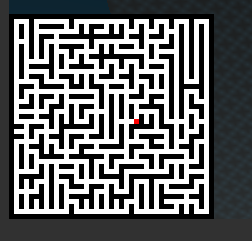
\includegraphics[width=0.8\textwidth]{Carte2020.png}
    \caption{Un exemple de carte possible (en rouge, la position du joueur)}
    \label{Un exemple de carte possible (en rouge, la position du joueur)}
\end{figure}

\paragraph{Affichage et Disparition de la Carte}
Concernant son affichage, il m'a fallu plus de temps. J'attendais de la Carte qu'en plus d'afficher le plan du complexe, elle affiche la position du Joueur la détenant en temps réel, afin de lui fournir de véritables indications. J'ai donc dû effectuer de nombreux tests, pour faire en sorte que la carte ne soit pas affichée au début dans un premier temps, puisque Unity affiche les images par défaut, et ensuite pour mettre au point le curseur sur la Carte, l'actualiser en fonction de la position du Joueur et le décaler en fonction de cette position et par rapport à la Carte. La difficulté, ici, est évidemment que l'affichage de la carte est simplifié et ne prend pas en compte la position exacte des murs. Autrement dit, affecter au Curseur une bête position directement proportionnelle aux coordonnées du Joueur ne suffit pas ; il me fallait plutôt déterminer la salle où le Joueur se trouvait. C'est cette partie qui m'a pris le plus de temps, car une erreur de quelques centimètres peut afficher le Joueur de l'autre côté d'un mur qu'il n'a pourtant pas franchi. Mais heureusement, tout fonctionne actuellement à merveille. J'ai également pris soin de laisser une fonction permettant d'effacer la Carte au besoin.

\paragraph{Objets de base}
Une fois que la Carte a été achevée, je suis alors passé au développement de cinq Objets basiques. Les Bottes de Pégase, qui donne au Joueur une vitesse deux fois plus importante que la normale, les Bottes de Plomb, qui lui donnent au contraire une vitesse deux fois moins importante que la normale, la Carte, qui affiche évidemment la Carte, la Paralysie, qui l'immobilise un faible instant, et la Décharge, qui lui retire tous les Objets qu'il conserve sur lui. Il y avait donc trois Objets à effets constants et deux à effets immédiats. Pour les Bottes de Pégase et les Bottes de Plomb, il m'a suffit d'affecter une valeur à un ratio de vitesse que Célian avait laissé comme propriété sur les Joueurs. Pour la Carte, je n'avais plus qu'à lancer la fonction d'affichage de cette dernière, et pour la Paralysie, à baisser la valeur "Stamina" à 0, pour simuler le choc lorsqu'un autre Joueur vout frappe. Pour la Décharge, il me suffisait donc de mettre à false tous les éléments du tableau des Objets constants, de lancer la fonction annulant l'affichage de la carte, et de rétablir la vitesse à son ratio normal. Bien sûr, comme indiqué précédemment, un Joueur ne peut pas prendre de Bottes de Pégase s'il en a déjà sur lui. Cela dit, j'ai fait en sorte que le Joueur puisse récupérer des Bottes de Plomb lorsqu'il a les Bottes de Pégase, et ainsi de suite. L'Objet ainsi récupéré devient alors tout de suite effectif, au lieu de simplement rétablir la vitesse du Joueur à sa vitesse normale. Autrement dit, si vous avez les Bottes de Plomb et que vous récupérez des Bottes de Pégase, vous avancerez quatre fois plus vite par rapport à la vitesse que vous aviez. J'ai également fait attention à ce que les Objets du Joueur se réactualisent à chaque fois qu'il prend un Objet.

\paragraph{Deuxième vague d'Objets}
Suite à ces cinq Objets, je me suis lancé dans la confection de trois autres Objets de cet acabit : la Disparition, la Protection, et le Casque de CRS. Ces trois Objets sont à effets constants. La Protection a un effet très simple, elle permet d'annuler l'effet d'un Objet à effet négatif. Il s'agit donc juste d'un effet à prendre en compte lors de l'application des effets des différents Objets. La Disparition, elle, permet à un joueur Guéri en seconde phase de devenir invisible pendant quinze secondes. Il devient alors inconsistant : il ne peut être infecté durant ce labs de temps, mais il ne peut pas non plus prendre d'Objets. Le Casque de CRS, lui, dissimule le labyrinthe au Joueur, qui doit donc avancer à l'aveuglette pendant quinze secondes, le temps de retirer le Casque. Ces deux Objets m'ont donné plus de fil à retordre que les autres. En effet, je souhaitais faire en sorte que les quinze secondes puissent être interrompues, avec l'effet qui cesse, en vue de la Décharge. Evidemment, ce n'était pas nécessaire pour la Disparition, mais plus pour le Casque de CRS. 

\paragraph{Développement d'un chronomètre désactivable}
Pour cela, j'ai fait en sorte que le "chronomètre" soit constitué d'un entier indiquant le temps restant en seconde et d'un booléen indiquant si une seconde était en train d'être comptée. Ainsi, à chaque image du jeu, je vérifiais que la seconde aie terminé d'être comptée. Si c'était le cas, je relançais une seconde, sinon je ne faisais rien. Et ainsi de suite, jusqu'à ce que le nombre de secondes tombe à 0. Dans ce cas, je lançais automatiquement l'arrêt de l'effet. Ainsi, pour désactiver un Casque de CRS quand on se prend une Décharge, il suffit simplement de baisser le nombre de secondes restantes à 0. De plus, quand le compteur passe à 0, je prenais soin de retirer l'Objet en question du tableau des Objets du Joueur, et de remettre à jour l'affichage de ces valeurs à l'écran. Concernant le Casque de CRS, j'avais également voulu le faire au départ un simple affichage de rectangle noir avec la propriété OnGUI de Unity. Le soucis, c'est qu'avec cette méthode, on ne voyait ni le nom du Joueur, ni son état, ni le temps qu'il restait avant la fin de la Partie, ni la Carte s'il l'avait, ni le message comme quoi le Joueur avait reçu le Casque de CRS, ni la liste des Objets que le Joueur avait. J'ai donc dû me résoudre à utiliser une Image, pour pouvoir la reléguer en arrière-plan, entre l'image du dédale et les différents éléments constituant l'écran du Joueur. J'ai ensuite dû faire en sorte que l'affichage noir lié à la présence automatique du Casque par Unity disparaisse au début du jeu pour chaque Joueur. On en est donc à huit Objets.

\begin{figure}[H]
    \centering
    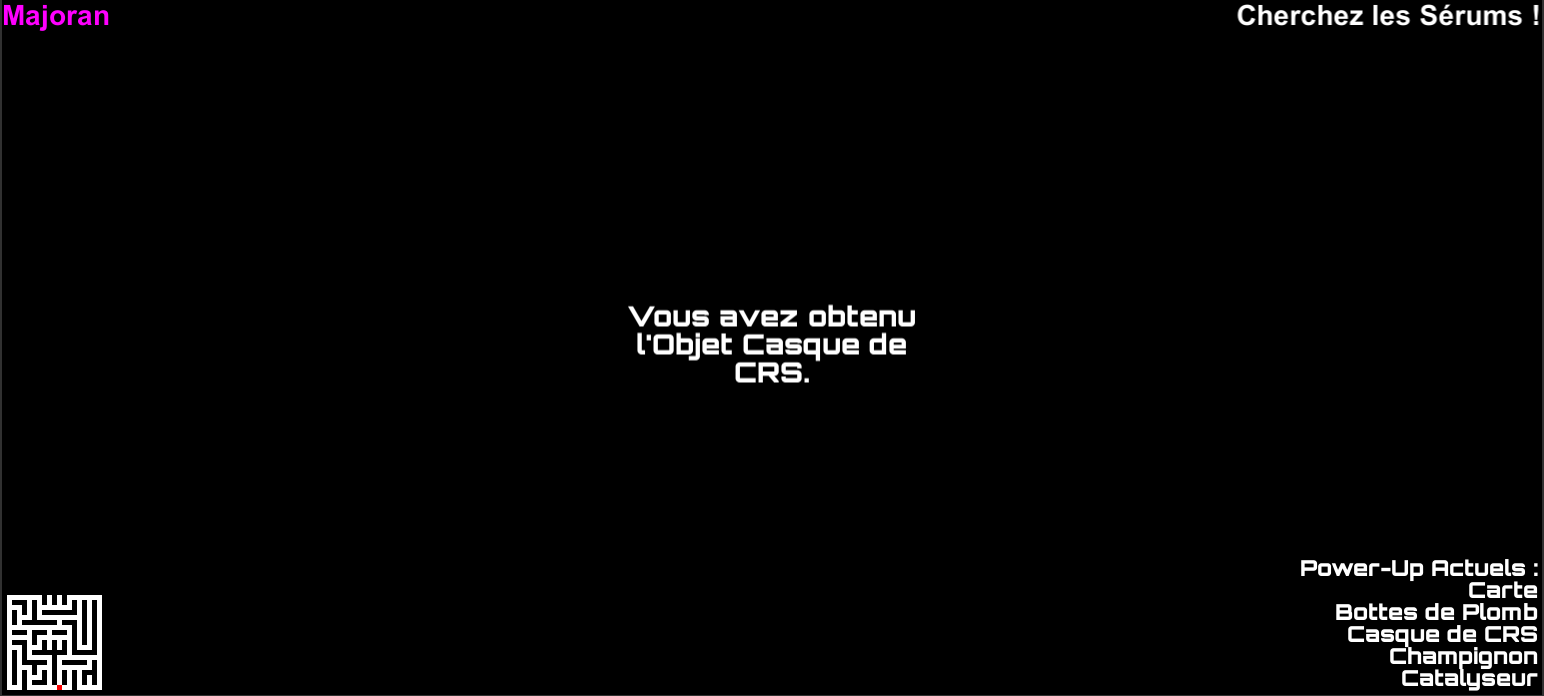
\includegraphics[width=0.8\textwidth]{Casque.png}
    \caption{Avec le Casque de CRS, seuls les textes sont encore visibles.}
    \label{Avec le Casque de CRS, seuls les textes sont encore visibles.}
\end{figure}

\paragraph{Dernière vague d'Objets}
Les cinq Objets restants, je les ai implémenté avec plus de facilité que les précédents. Il s'agit du Champignon, du Sérum d'Urgence, de l'Herbe Bleue, du Catalyseur et des Ressorts. Le Champignon et les Ressorts sont des Objets Inutiles : le Champignon vous assène simplement des sons particuliers dans votre oreillette, à la manière d'hallucinations sonores, et les Ressorts vous font sauter automatiquement pendant quelques secondes. Etant donné que je savais déjà comment évaluer ce type de chronomètre, les Ressorts ont été relativement simples à encoder. Pour le Champignon, j'ai en revanche dû m'arranger avec Célian pour comprendre la manière dont il avait inséré les sons dans le programme. Le Catalyseur, lui, est un Objet à effet négatif qui reste jusqu'à ce que vous vous preniez une Décharge : il double tout simplement le temps de récupération après une Paralysie, que ce soit déclenché par l'Objet Paralysie ou par un autre Joueur. Quant au Sérum d'Urgence et à l'Herbe Bleue, ils ont été plus intéressants à développer. Pour commencer, ces deux Objets ne peuvent être récupérés qu'en seconde phase. Le premier, en plus, ne peut être pris que par un Joueur Guéri. Le Sérum d'Urgence permet à un Joueur Guéri de disparaître quand il se fait infecté. Autrement dit, quand un Joueur Condamné effleure le Joueur Guéri ayant ce Sérum d'Urgence, il a la surprise de voir ce Joueur disparaître au lieu de devenir simplement un nouveau Condamné. Le Joueur qui vient de disparaître, quant à lui, dispose de cinq secondes avant de redevenir visible, et donc de nouveau infectable. On peut donc considérer qu'il s'agit d'une vie supplémentaire.

\paragraph{L'Herbe Bleue, un Objet Commun}
L'Herbe Bleue, elle, est un Objet Commun. Autrement dit, quand un Joueur ramasse une Herbe Bleue, l'effet s'applique sur tout le monde. En effet, l'Herbe Bleue rallonge de trente secondes la durée de la seconde phase. Pour implémenter ces deux Objets, il m'a donc fallu comprendre où se déroulait l'infection d'un Joueur, et faire en sorte de pouvoir rallonger le temps de la seconde phase tout en affichant un message aux autres Joueurs pour les prévenir de ce détail. Pour le Sérum d'Urgence, j'ai donc regardé du côté de la fonction que Célian utilisait pour faire changer un Joueur d'état. Dans le cas où le nouvel état était l'état de Condamné, il m'a donc suffit de rajouter la condition de la présence du Sérum d'Urgence dans les Objets de Joueur en question. S'il en avait un, il ne me restait plus qu'à faire en sorte que l'état dans lequel il serait serait l'état d'invisible au lieu de Condamné, et de lancer en même temps un chronomètre de cinq secondes pour rétablir l'état Guéri du Joueur plus tard. J'ai procédé de la même manière pour l'Herbe Bleue : j'ai rendu la variable des chronomètres de seconde phase des Joueurs directement accessible via le script PlayerNetwork, où sont effectuées la majorité des fonctions en réseau. Ainsi, quand quelqu'un reçoit une Herbe Bleue, il lui suffit de lancer la fonction en réseau correspondante. Et quand un Joueur reçoit cette fonction, le chronomètre augmente de trente secondes. Avec, bien sûr, un petit message sur son écran dans le cas où il ne s'agirait pas du Joueur ayant récupéré ledit Objet.

\begin{figure}[H]
    \centering
    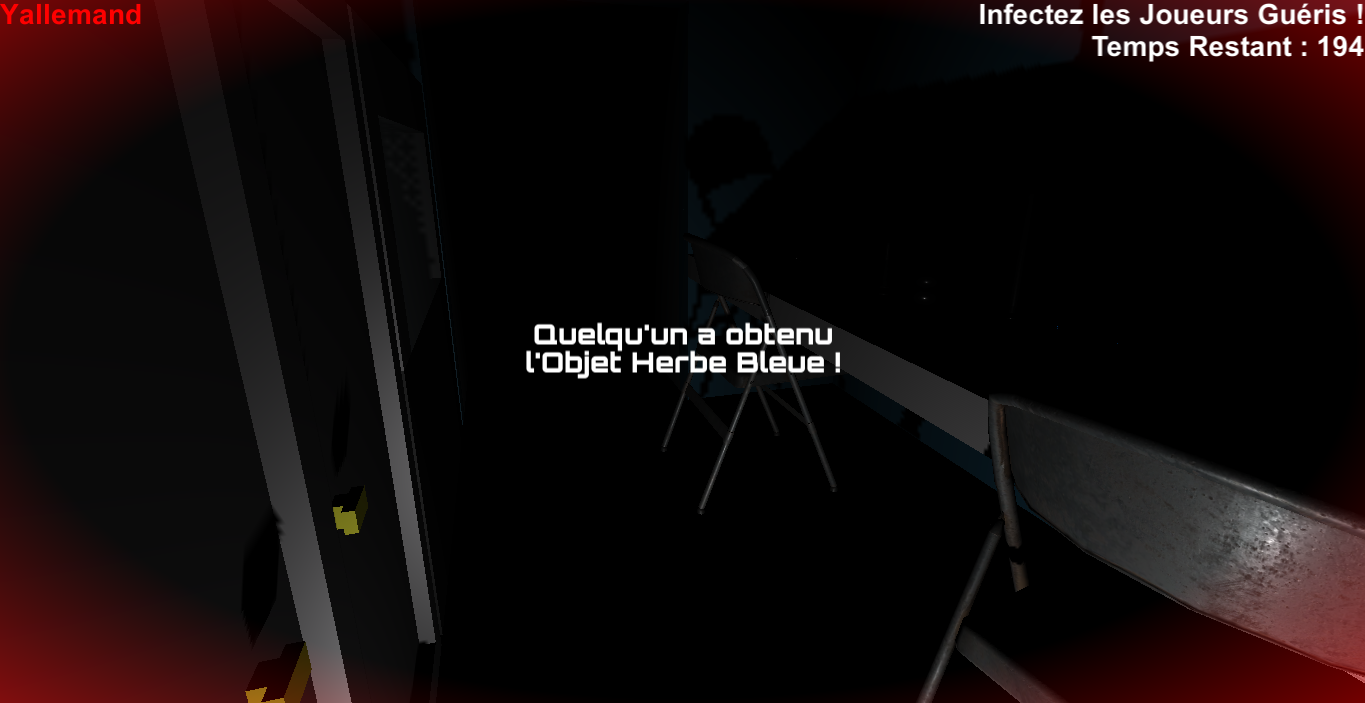
\includegraphics[width=0.8\textwidth]{MessageHerbeBleue.png}
    \caption{Comme l'Herbe Bleue est un Objet Commun, un message alerte les autres joueurs si quelqu'un en ramasse...}
    \label{Comme l'Herbe Bleue est un Objet Commun, un message alerte les autres joueurs si quelqu'un en ramasse...}
\end{figure}


\newpage
\section{Réalisations}
En ce qui concerne l'ambiance du groupe, il n'a pas eu durant la totalité du projet d'importantes discordes, vu que les travaux attendus ont toujours été donné à temps.

\subsection{Nos peines}
L'une des plus grosses peines fut causée par Photon. A chaque fois que l'on voulait synchroniser quelque chose dans le réseau, c'était un défi. Par exemple, vers le milieu de la première soutenance, on a du refaire toute la structure du réseau car les méthodes et variables utilisées n'était disponibles que sur une version antérieure, ce qui nous a déjà fait perdre plus de 15 heures de travail. A chaque fois que l'on voulait ajouter une fonctionnalité sur le jeu, il fallait quasiment autant de temps pour la faire que pour la synchroniser sur le réseau. Mais malgré cela, avec persévérance et courage, nous sommes arrivés à nos buts. Je pense que le plus gros défi du projet fut la génération des joueurs en réseau. Plus de 20 heures ont été mises pour chercher une solution simple, efficace et pratique pour celle-ci. On a changé plusieurs fois de systèmes, mais finalement on a abouti sur un système performant, simple et optimisé. 

Lors du dernier semestre, un autre défi fut de taille. Vu que l'on instancie les joueurs dans une scène différente de celle des menus, la scène ne comportait soit deux caméras pour chaque joueur, soit aucune. Donc il a fallu regarder une à une chacune des méthodes pour voir à quel exact moment les caméras sont crées pour ne pas avoir de doublons. Ce fut extrêment long et fastidieux vu que le jeu tourne normalement à 60 FPS, c'est-à-dire 60 images par seconde. Donc il falllait regarder images par images, là où il fallait la détruire et là où créer la nouvelle. Ce ne fut pas particulièrement dur, mais surtout long et fastidieux.

En dehors de ça, il a fallu juste corriger les différents bugs qui arrivé lors du dévellopement du jeu ou des phases de test, mais globalement, il n'y a pas eu de grandes peines. On a fallit avoir des problèmes de fusion de stockage avec Git mais grâce à la connaissance de Git par Célian, tout s'est bien passé.

\subsection{Nos joies}
Chacune de nos avancés sur le projet fut une joie en soi. Le fait de travailler dur et longtemps sur un système et de le voir marché est très jouissif. Par exemple, Célian a grandement apprécié travaillé sur les shaders du jeu. Steve, lui a aimé voir le réseau marchait correctement et les animations fluides en réseaux. 

Lors de la création du cahier des charges, on a cru que la plupart du temps du projet se serait consacré à la génération aléatoire du labyrinthe, vu que l'algorithme le gérant ne fut pas encore vu en cours. Mais finalement, Léandre y est arrivé très facilement. Le plus intéressant dans tout cela, c'est que lorsque l'on a eu des cours nous expliquant les différents algorithmes de génération de labyrinthe, la version de Léandre fut quasiment la même de celle de Prim, qui est très optimisée, alors qu'il n'en avait même pas connaissance. 

Dès la deuxième soutenance, le jeu était désormais totalement jouable et je pense que ce fut notre plus grande joie pour ce projet. Le fait de voir tous nos travaux marcher ensemble et comme attendus, fut très gratifiant. On sentait que malgré la complexité des mécanismes internes utilisés, le jeu était très amusant à jouer. On s'est aussi rendu compte qu'il y'avait plusieurs statégies pour joueur, ceux qui préféraient se cacher et ramasser peu d'objets pour ne rien risquer, et à l'inverse, ceux qui courraient dans tout le labyrinthe à prendre tous les objets, bon ou mauvais.

De plus, le système de combat a rajouté une nouvelle dimension au jeu : fallait-il aller au combat pour ralentir les autres joueurs ou bien fuir pour ne pas se voir immobiliser ? Globalement, le jeu fut dans sa grande majorité une immense joie à nos yeux. Il nous a fait progressé en programmation, nous a appris l'esprit et le travail d'équipe et nous a renforcé.

\newpage
\section{Conclusion}

En un semestre, nous avons ainsi réussi, en-dehors du cadre des cours et d'un petit problème de confinement, à réaliser un jeu en multijoueur sur Unity, tout en amassant des connaissances nécessaires à l'élaboration de ce projet. Le jeu que nous vous avions présenté lors de la seconde soutenance était déjà parfaitement jouable, mais actuellement, "Deadly Science" est désormais net, propre, avec de nombreuses options rajoutées pour faciliter la vie aux joueurs ou, au contraire, renforcer son immersion. Dire que nous ne sommes pas satisfaits du travail que nous avons fourni et du jeu que nous vous avons fourni serait absolument faux.

En effet, loin de nous être contentés de suivre le cahier des charges, nous avons pu aller plus loin que les objectifs que nous nous étions fixés en rajoutant la possibilité de choisir un mode, de prendre des objets, de choisir le nombre de joueurs, ou même de modifier la taille du labyrinthe. Durant tout le projet, nous avons été en avance sur nos prédictions concernant l'évolution du jeu.

Nous espérons donc que vous prendrez du plaisir à vous égarer dans les couloirs tortueux de "Deadly Science", à la recherche de votre rédemption ou de votre vengeance. Mais quoi qu'il en soit, le jeu est loin d'être totalement terminé ; nous comptons, même dans un cadre hors-soutenance, continuer à rajouter des objets, des salles, des modes, ou tout simplement des musiques. En un mot comme en mille, vous n'avez pas terminé de découvrir les bas-fonds des laboratoires de Deadly-Science !

\subsection{Sources et remerciements}

Beaucoup d'éléments du jeu ont été conçus par nos soins, certains d'entre eux ont été créés par d'autres personnes que nous remercions car sans elles notre jeu ne serait pas aussi bien.

\begin{itemize}
    \item Animations : Basic Motion Pack (Assets Store) par Kevin Iglesias
    %%% TODO : Modele
    \item Réseau : Photon
    \item Effets sonores : Tous les sons ont été trouvés sur freesound.org
\end{itemize}
    
%%% TODO : Reformuler
Nous tenons également à remercier toutes les personnes ayant contribuées aux outils gratuits ou open source que nous avons utilisés.
Et enfin, un grand merci aux testeurs et examinateurs du jeu.


\newpage
\begin{center}
\emph{If you knew time as well as I do, you would play Deadly Science.}
\end{center}

\end{document}



